% !TeX root = bachelorarbeit.tex

\subsection{Modellproblem}

In diesem Abschnitt wollen wir anhand des linearen Transportproblems auch tatsächliche praktische Resultate der Multilevel Monte Carlo Methode beleuchten.
Wir setzen dazu
\begin{itemize}
	\item $ \mathcal{D} = (0,1)^2 \subset \R^2 $ (also insbesondere wie breits zuvor in der Theorie $ n=2 $)
	\item $ \mathbb{T} = [0,T] = [0,1] $ (vgl. Bemerkung \ref{wahlfunk})
	\item $ \rho_{\text{in}} \equiv 0 $
	\item $ \rho_0(x) = 
	\begin{cases*}
		\begin{array}{llll}
			&c & , &\text{für }x \in B \coloneqq [0.2,0.8] \times [0.775 ,0.825]  \\
			&c\exp \left(\frac{ \left| \frac{\text{dist}(x,B)}{0.12} \right| ^2}{\left|\frac{\text{dist}(x,B)}{0.12}\right|^2-1}\right) &, &\text{falls } \text{dist}(x,B)>0.12 \\
			&0 &, & \text{sonst}
		\end{array}
	\end{cases*}$ \\
	Dabei sei $ c $ so gewählt, dass 
	\[
		\int_{\mathcal{D}} \rho_0(x) \dx = 1 \ ,
	\]
	wir skalieren also die zur Beginn im Rechengebiet enthaltene Masse auf $ 1 $.
\end{itemize} 
Die Anfangskonzentration $ \rho_0 $ entspricht also gerade einer rechteckigen Ansammlung mit Länge $ 0.6$ und Breite $ 0.1$ und Mittelpunkt $ (0.5,0.75) $, welcher in beide Richtungen auf einem $ 0.15$ breiten Streifen mit einer Exponentialfunktion in die Ebene geglättet wird. 
Wir stellen so für die Anfangsbedingungen unseres Modellproblems einen sehr hohen Grad an Regularität sicher. 
Visuell kann diese Anfangskonzentration folgendermaßen dargestellt werden:
\begin{figure}[H]
	\centering
	\captionabove{Anfangsbedingung $ \rho_0 $}
	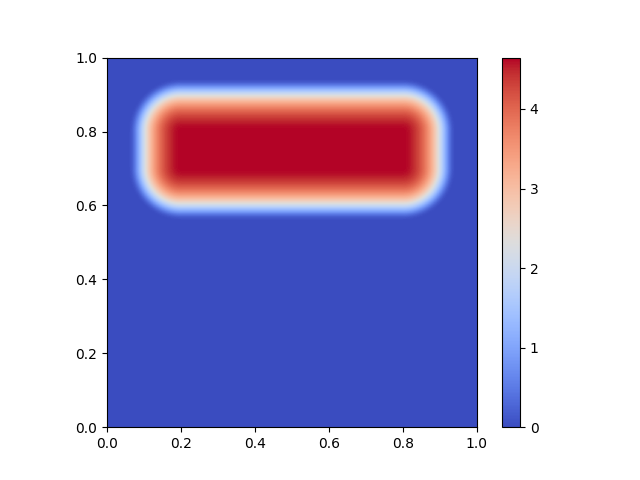
\includegraphics[width=0.65\textwidth]{plots/anfangsbedingung.png} 
\end{figure}
Der Maximalwert ist dabei so gewählt, dass die Gesamtmasse der Anfangsbedingung gerade den Wert $ 1 $ ergibt.\\
Uns interessiert nun folgende Fragestellung: \\
\textbf{Wie groß ist der erwartete Anteil der Masse, welcher nach Ablauf des betrachteten Zeitintervalls $ \mathbb{T} $ im Rechengebiet $ \mathcal{D} $ verbleibt?}\\

Wie bereits an früherer Stelle erklärt, berechnen wir hierzu ein stochastische Flussvektorfeld $ q : \Omega \times \overline{\mathcal{ D}} \to \R^2 $ als Lösung des zugehörigen Potentialströmungsproblems, wobei wir dabei den Permeabilitätstensor $ \kappa : \Omega \times \mathcal{D} \to \R_{\geq0} $ als lognormal verteiltes Zufallsfeld modellieren. Wir identifizieren dabei die Verteilung von $ \kappa $ mit der zugehörigen Kovarianzfunktion:
\[
 C(x,y) = \sigma^2 \exp(- \frac{\lVert x-y \rVert_2^s}{\lambda^s} ) .
\]
Dabei ist $ 0 < \sigma^2 < \infty $ die Varianz des zugrundeliegenden Gauß'schen Zufallsfeldes, durch $ \lambda = (\lambda_1,\lambda_2) \in \R^2 $ werden die Korrelationslängen in die verschiedenen Koordinatenrichtungen gegeben und $ s \in (1,2) $ ist ein Glättungsparameter. \\
Wir können auch den das lognormal verteilte Zufallsfeld und das daraus resultierende stochastische Flussvektorfeld $ q $ exemplarisch für ein $ \omega \in \Omega $ grafisch darstellen. Bei der Visualisierung des Flussvektorfeldes nutzen wir dabei sogenannte 'Streamlines'. Im Wesentlichen nutzt man dabei einen Zeitintegrator, wie etwa ein Runge Kutta Verfahren, und integriert mit deren Hilfe an verschiedenen Ausgangspunkten entlang des Vektorfeldes.

\begin{figure}[H]
	\centering
	\captionabove{Visualisierung der stochastischen Modellierung}
	\subfigure[Streamlines des entstehenden Flussvektorfeldes]{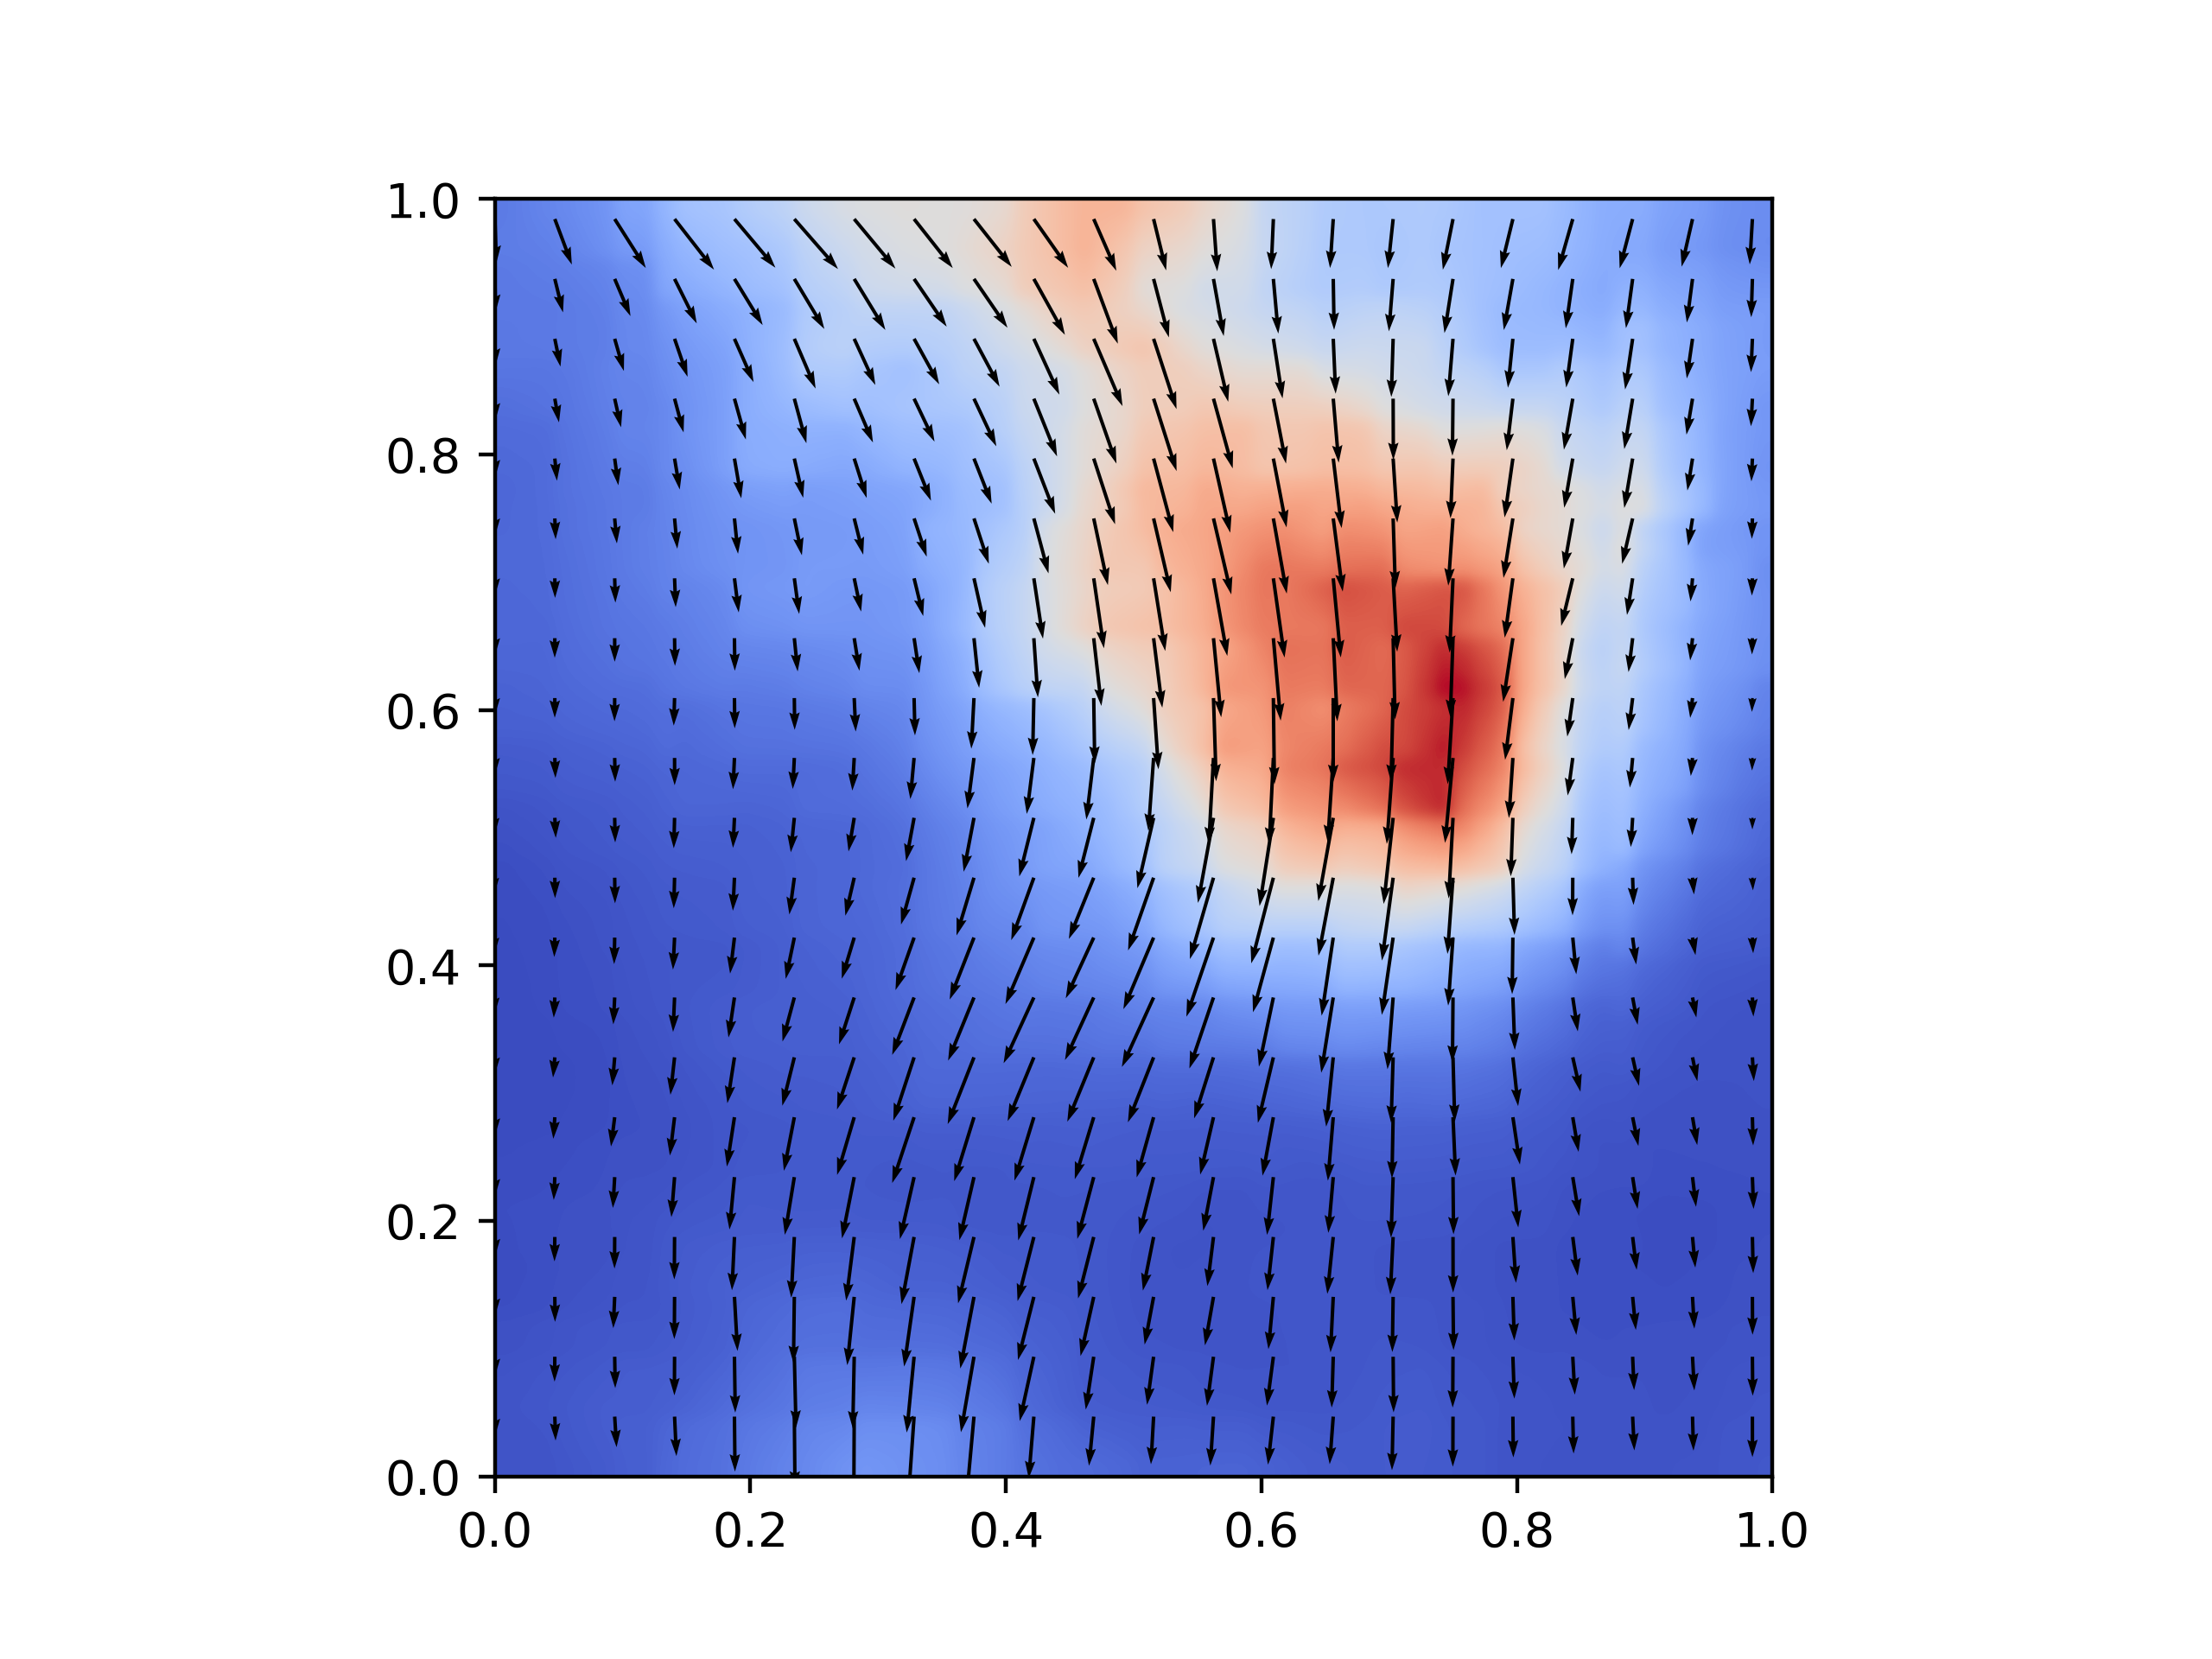
\includegraphics[width=0.49\textwidth]{plots/permquiv.png}}
	\subfigure[lognormal verteiltes Zufallsfeld mit obigen Parametern]{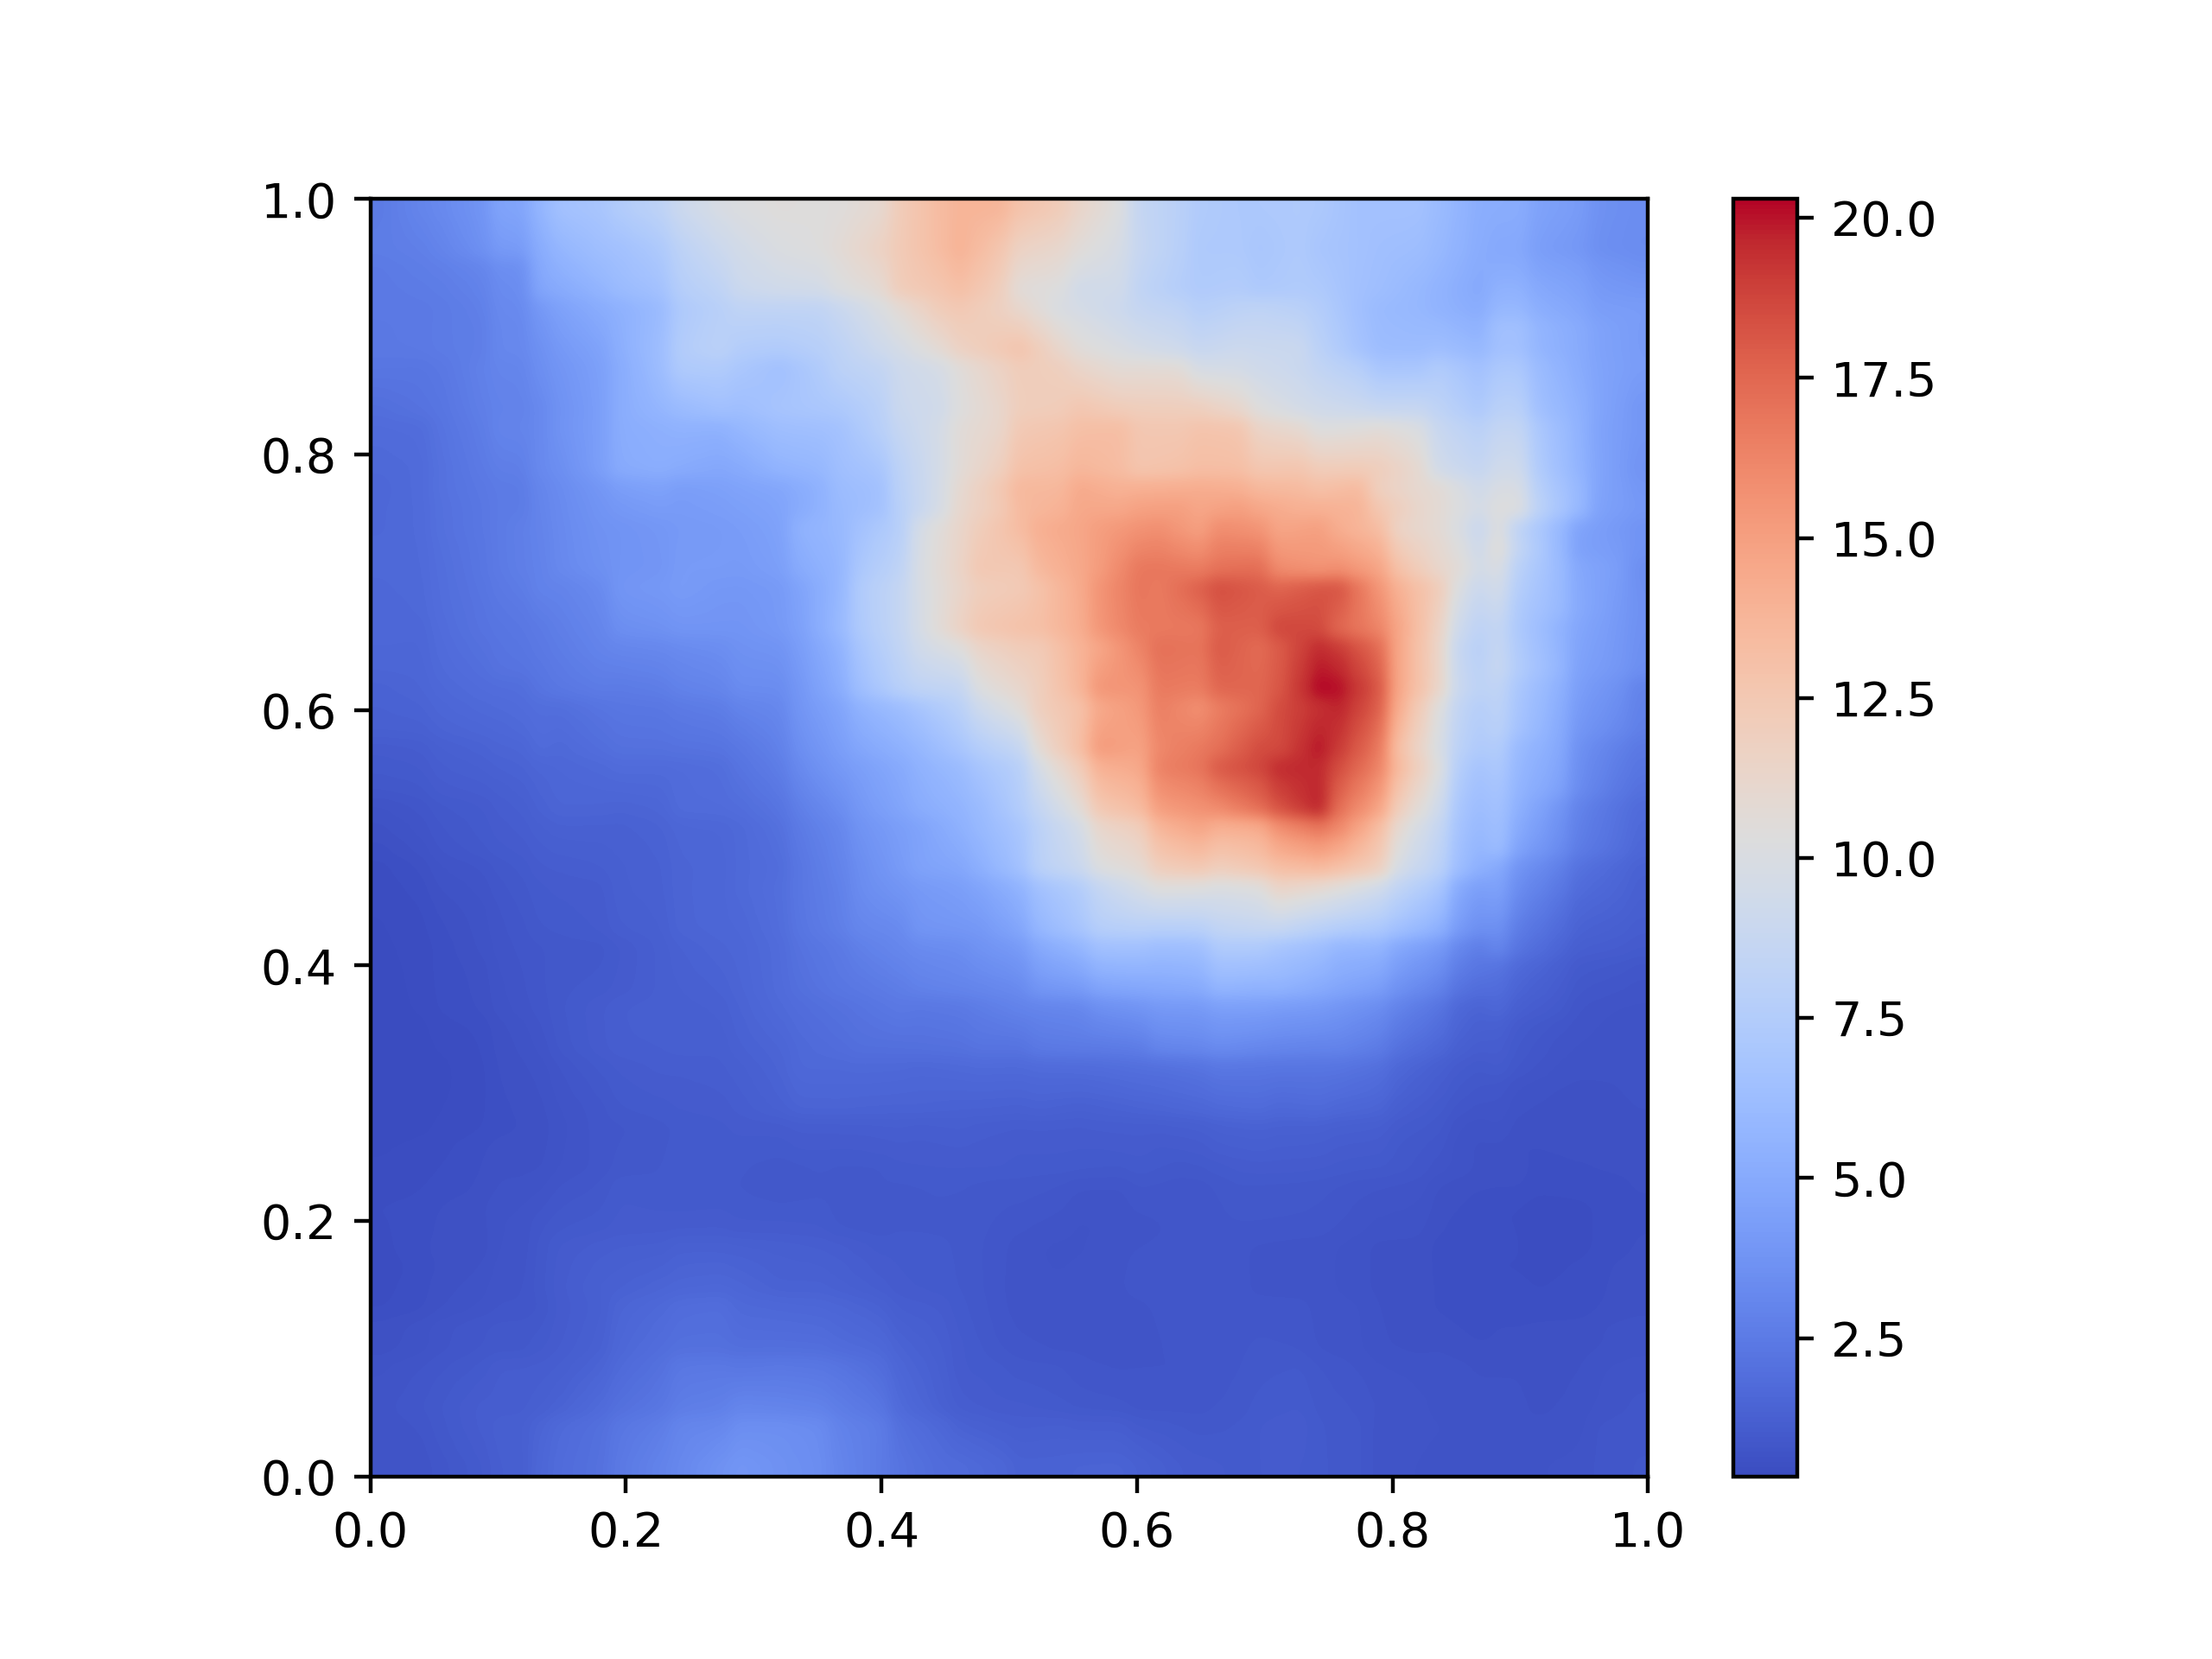
\includegraphics[width=0.49\textwidth]{plots/perm.png}}
	
\end{figure}

Weiter setzen wir
\begin{itemize}
	\item $\Gamma_{\text{D}} = \{ x = (x_1,x_2) \in \overline{\mathcal{D}} : x_2 = 0 \} $
	\item $ \Gamma_{\text{N}} = \partial \mathcal{D} \setminus \Gamma_{\text{D}} $
	\item $ g_N = \begin{cases}
						\begin{array}{llll}
						    &0 &, &\text{falls } x \in \{ x \in \Gamma_{\text{N}} : x_1 \in \{ 0,1 \}  \} \\
						    &1 &,& \text{sonst}
						\end{array}
				  \end{cases} $
	\item $ u_D \equiv 0 \text{ auf } \Gamma_{\text{D}} $
	
\end{itemize}

Als Zerlegung von $ \mathcal{D} $ wählen wir gleichartige Quadrate. Um auf dem geringsten Level ein Mindestmaß an Auflösung zu gewährleisten wählen wir auf Level $ l_0 $ eine Zerlegung in $ 256 = 16^2 $ Quadrate. Dies entspricht einer Ortsdiskretisierungsschrittweite von $ h_0 = \frac{1}{16} = 0.0625 $. Wie bereits im Theorieteil angemerkt, wählen wir von $ h_0 $ ausgehend die uniforme Familie von Zerlegungen $ \{\mathcal{T}_h \}_{h \in \mathcal{H}} $ mit $ \mathcal{H} = \{ h_0 , h_1 \coloneqq \frac{h_0}{2},h_2 \coloneqq \frac{h_1}{2} = \frac{h_0}{4}, \dots \} $. Auf Level $ l_1 $ betrachten wir also $ 1024 = 32^2 $ und auf Level $ l_k $ dementsprechend $ 2^{2(k+4)} $ Quadrate. 
In M++ entspricht Level $ l_0 $ bei der gewählten Diskretisierung 'UnitSquare' gerade Level $ 4 $. Die Zerlegungen auf $ l_0 = 4, l_1 = 5 $ und $ l_2 = 6 $ lassen sich folgendermaßen darstellen:
\begin{figure}[H]
	\centering
	\captionabove{Zerlegung des Gebietes $ \mathcal{D} $ in Finite Elemente}
	\subfigure[$l_0$ (256 Zellen)]{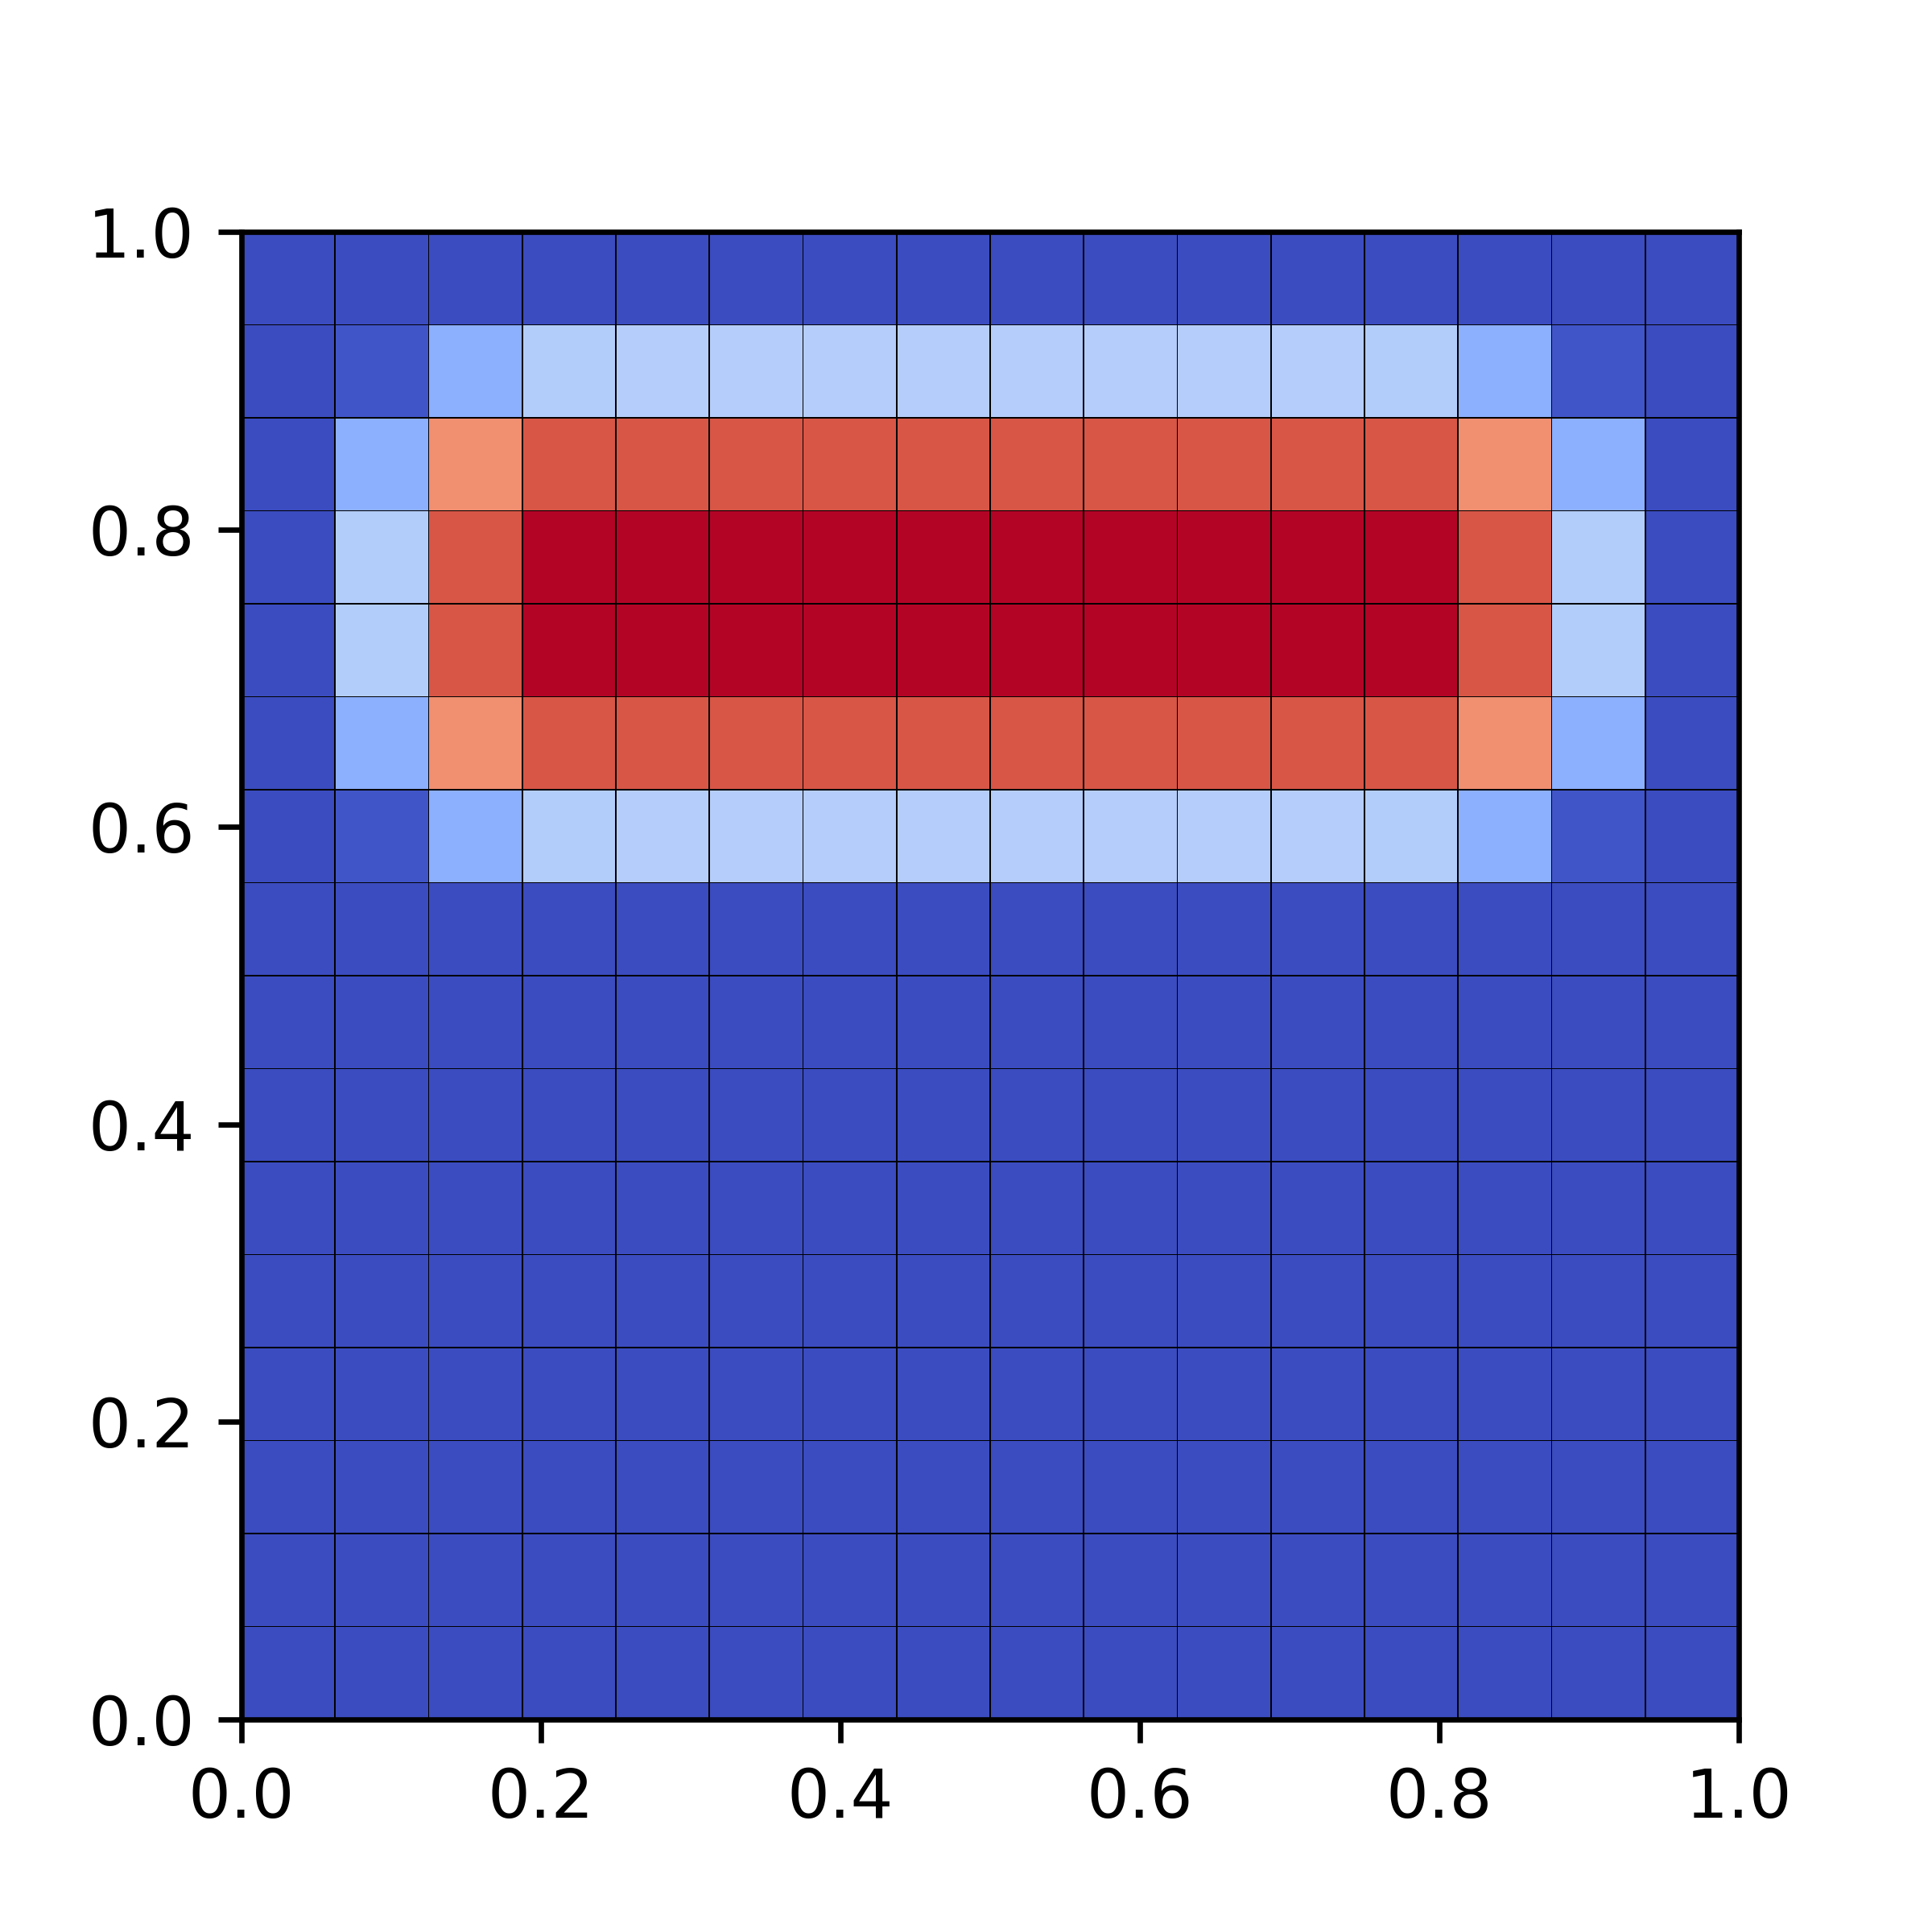
\includegraphics[width=0.31\textwidth]{plots/mesh4.png}}
	\subfigure[$l_1$ (1024 Zellen)]{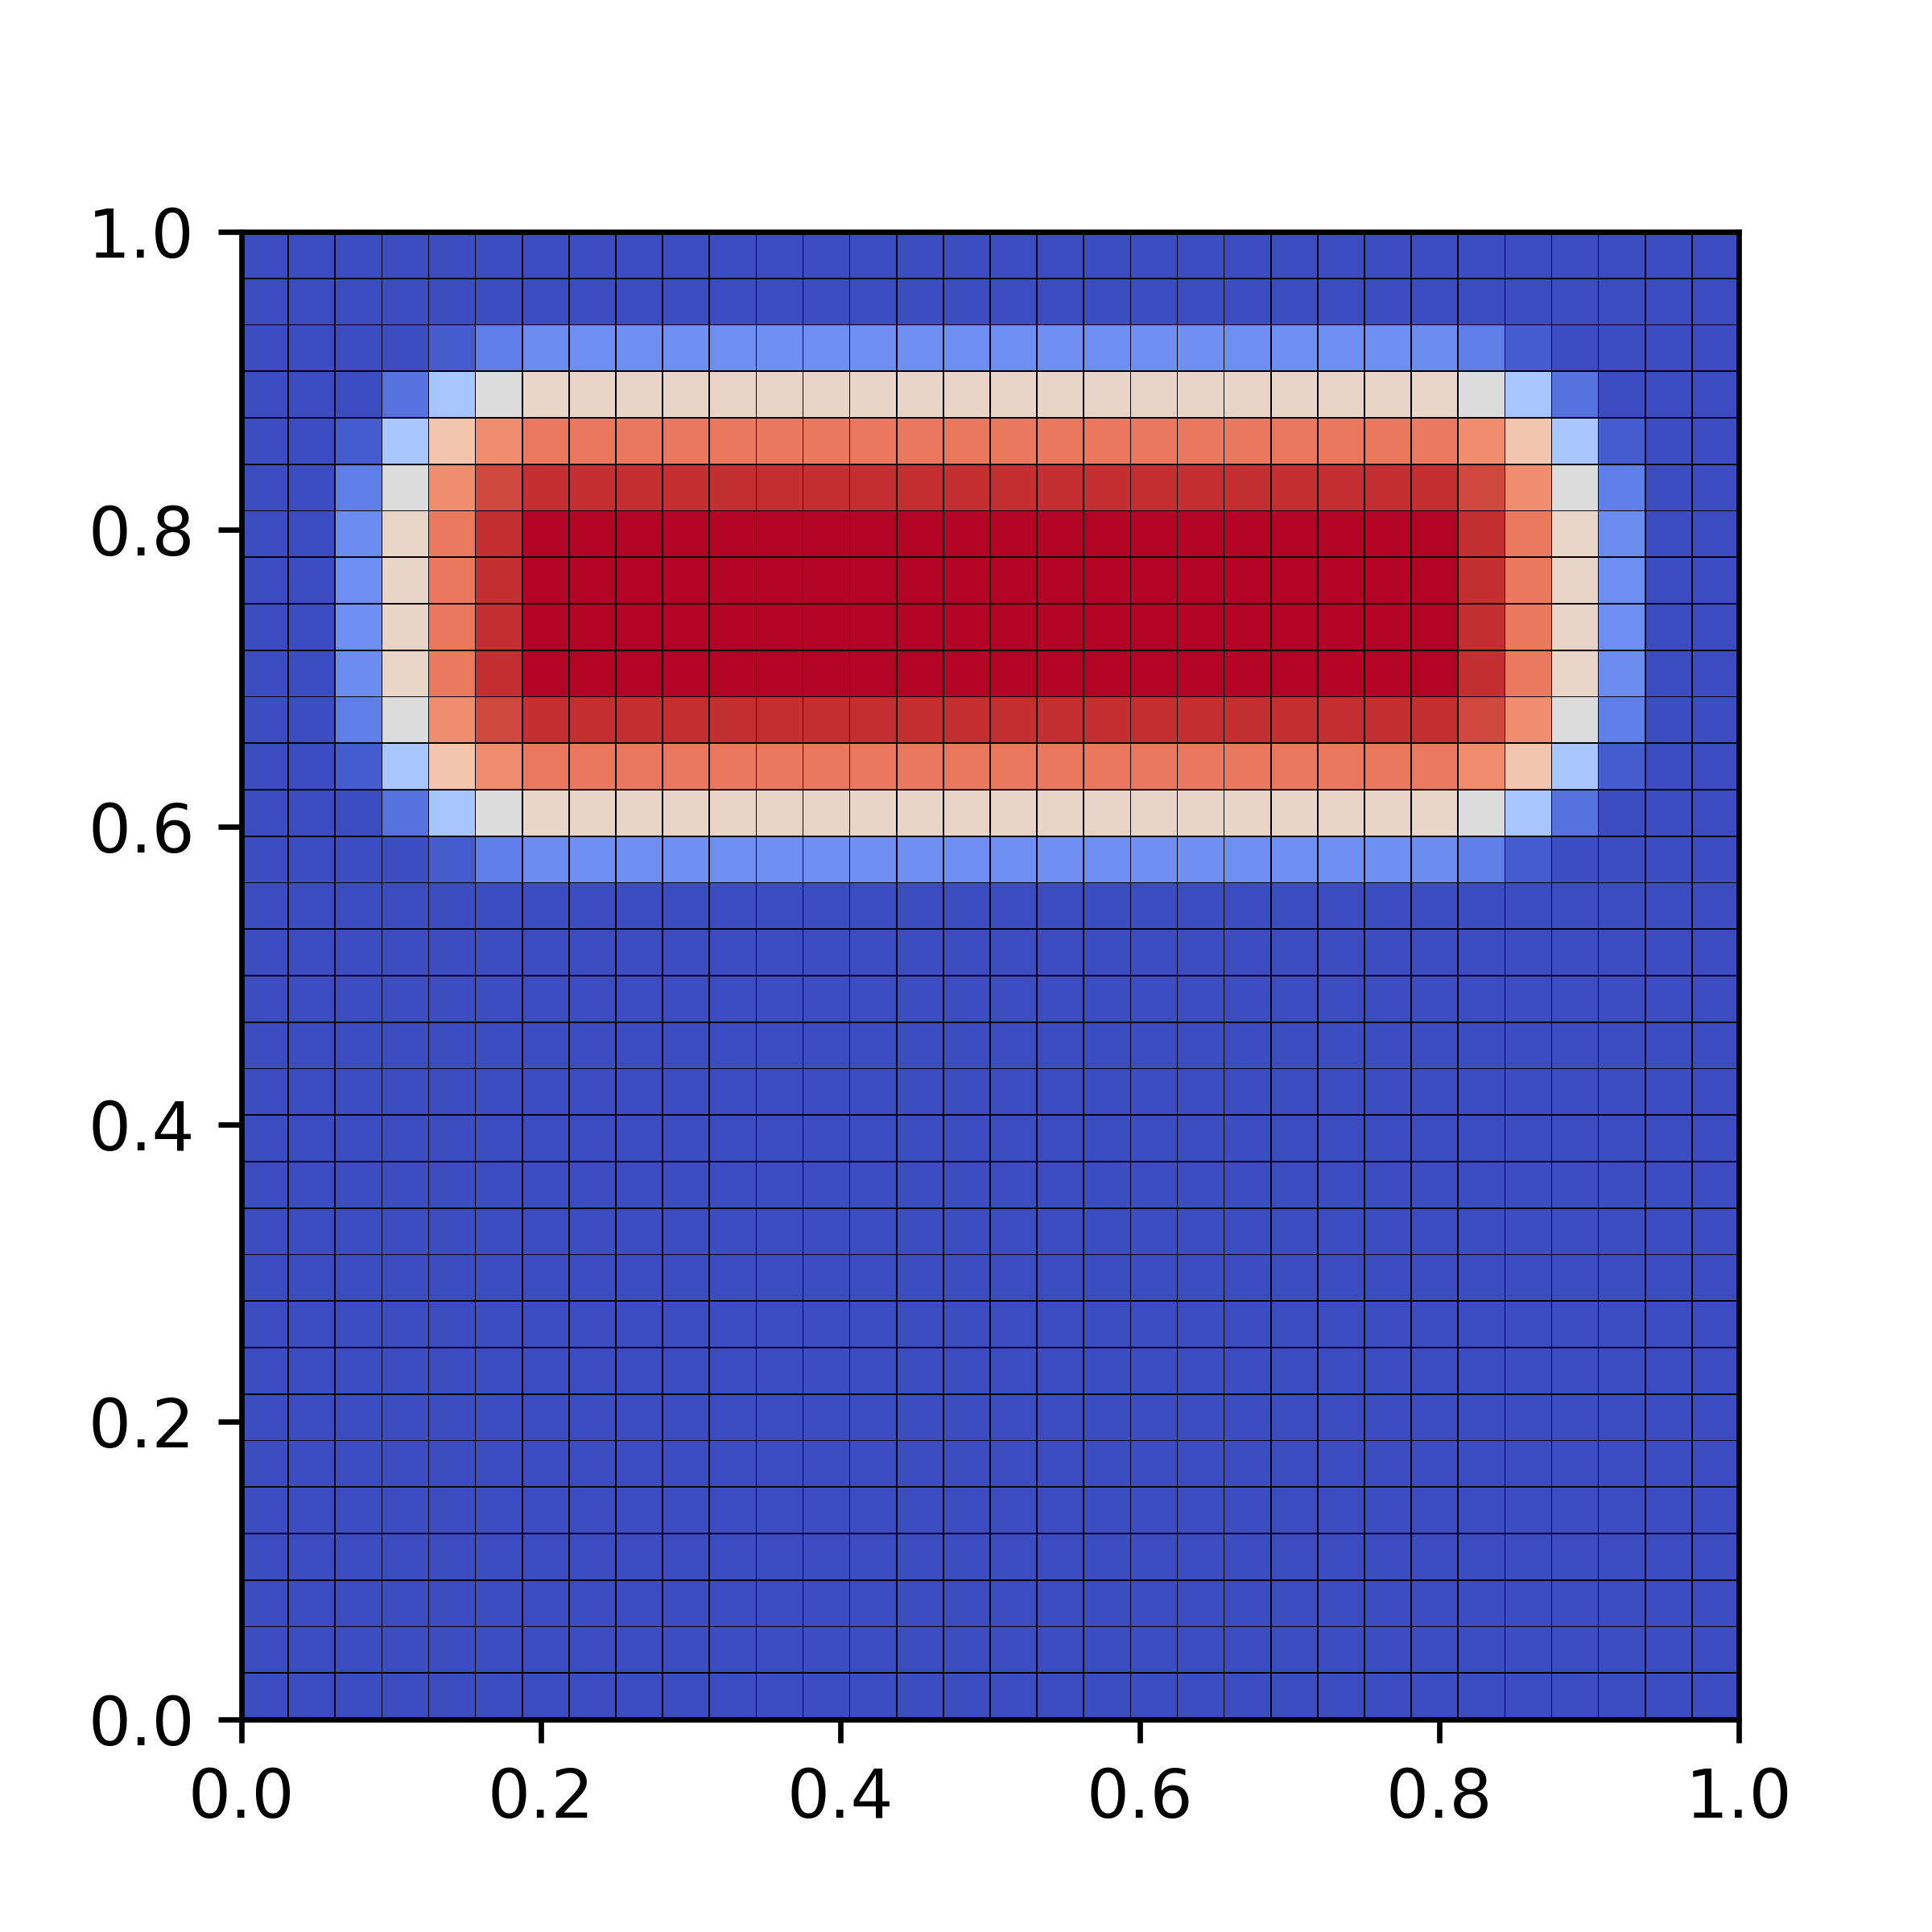
\includegraphics[width=0.31\textwidth]{plots/mesh5.png}}
	\subfigure[$l_2$ (4096 Zellen)]{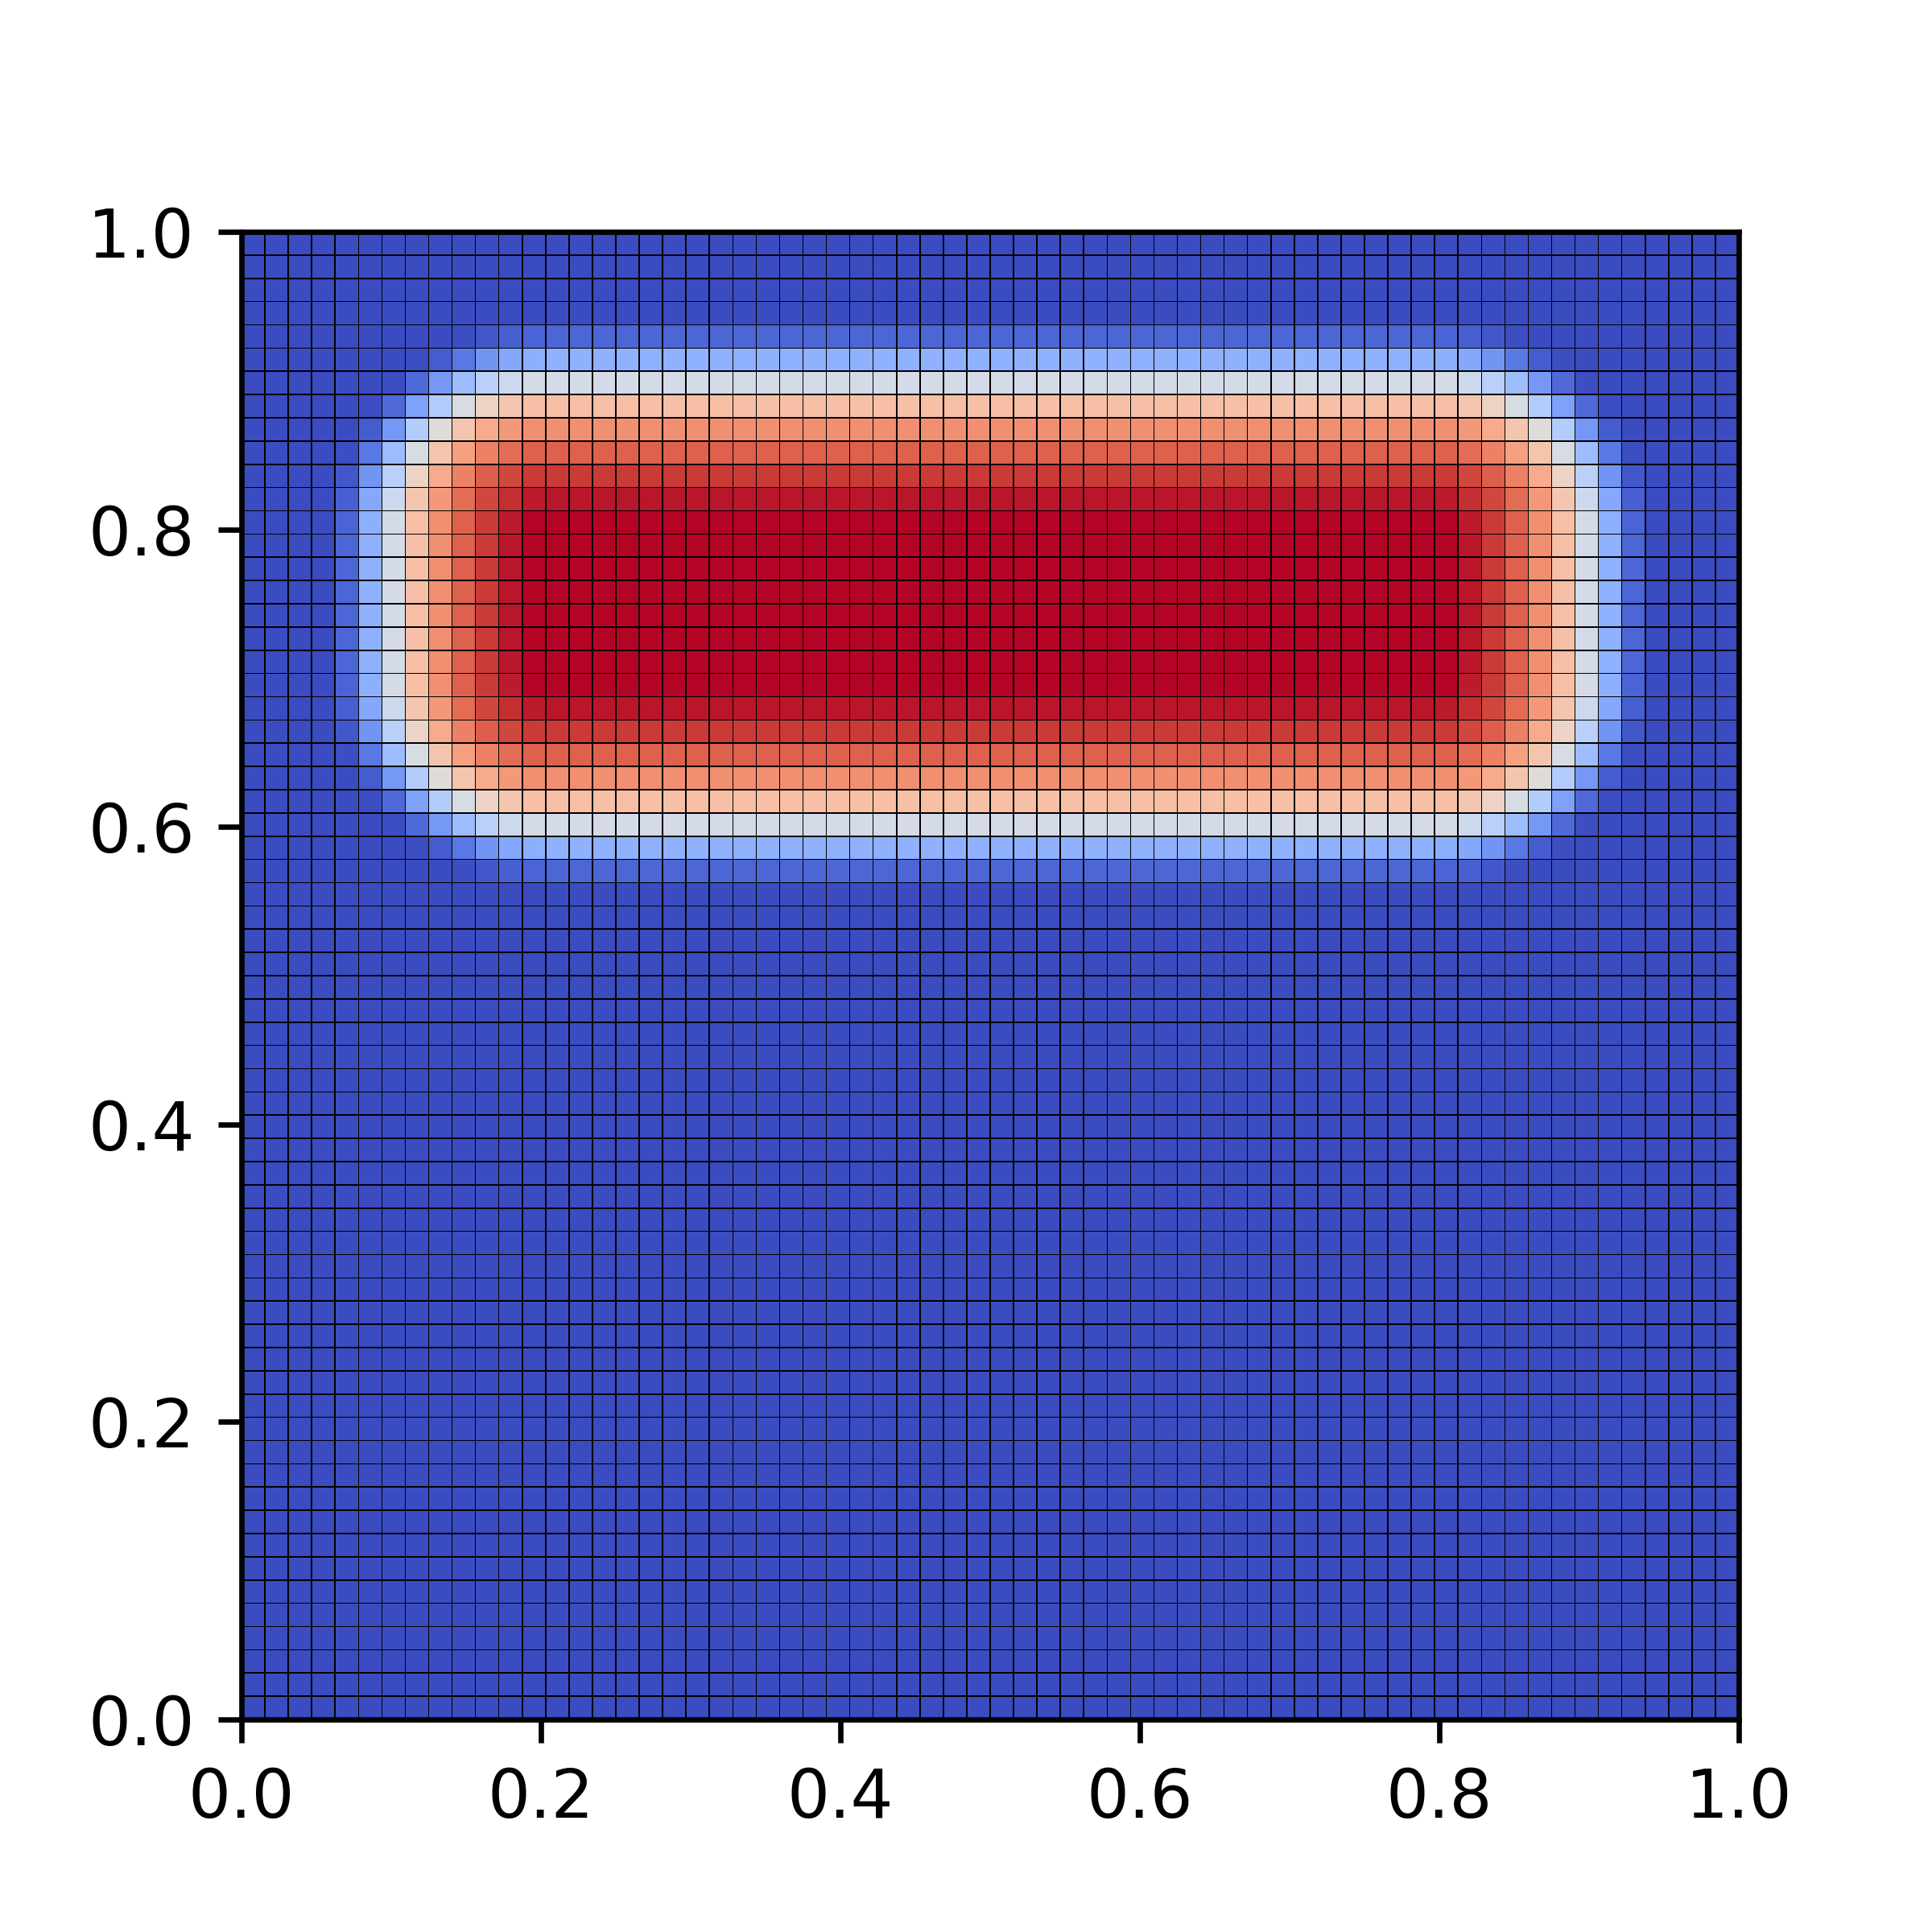
\includegraphics[width=0.31\textwidth]{plots/mesh6.png}}
\end{figure}
Die Schrittweite für die Diskretisierung in der Zeit setzen wir auf $ \Delta t = \frac{h}{8} $. Diese Wahl ist besonders hinsichtlich der Stabilität des Verfahrens wichtig. Bei zu kleinen Zeitschrittweiten treten Oszillationen in der Lösung auf. Obige Wahl hat sich für unser Problem als hinreichend erwiesen.
Entsprechend unserer Fragestellung können wir nun das betrachtete Zielfunktional formulieren:
\[
Q(\omega) = J(\rho(\omega)) \coloneqq \int_{\mathcal{D}} \rho(\omega,x,T) \dx = \int_{\mathcal{D}} \rho(\omega,x,1) \dx
\]
Wir suchen gemäß unserer Fragestellung also gerade nach $ \mathbb{E}[Q] $.
\begin{Bemerkung2}\label{wahlfunk}
	Die Wahl $ T=1 $ ist an dieser Stelle gerade so getroffen, dass das der Fragestellung entsprechende Zielfunktional in gewisser Weise interessant ist. 
	Genauer ist $ T $ so gewählt, dass die im Algorithmus auftretende Varianz $ \mathbb{V}[Y_l] $ 'groß' ausfällt. Ist $ T $ nämlich zu groß gewählt befindet sich für fast alle $ \omega \in \Omega $ kaum noch Masse im Gebiet und die erwartete Endmasse ist $ \mathbb{E}[Q] = 0 $, während für sehr kleine $ T $ Masse zum Zeitpunkt $ T $ für fast alle $ \omega \in \Omega $ mit der Anfangsmasse übereinstimmt und somit $ \mathbb{E}[Q] = 1$. Für $ T = 1 $ erhalten wir für verschiedene $ \omega \in \Omega $ recht unterschiedliche Ergebnisse, da die Masse je nach Beschaffenheit des Flussvektorfeldes schneller oder langsamer durch das Gebiet transportiert wird. 
\end{Bemerkung2}
Einen guten kompakten Überblick über ein einzelnes Sample bietet folgende Darstellung:
\begin{figure}[H]
	\centering
	\captionabove{Verlauf der Konzentration eines Beispielsamples auf Level $ l_3=7 $}
	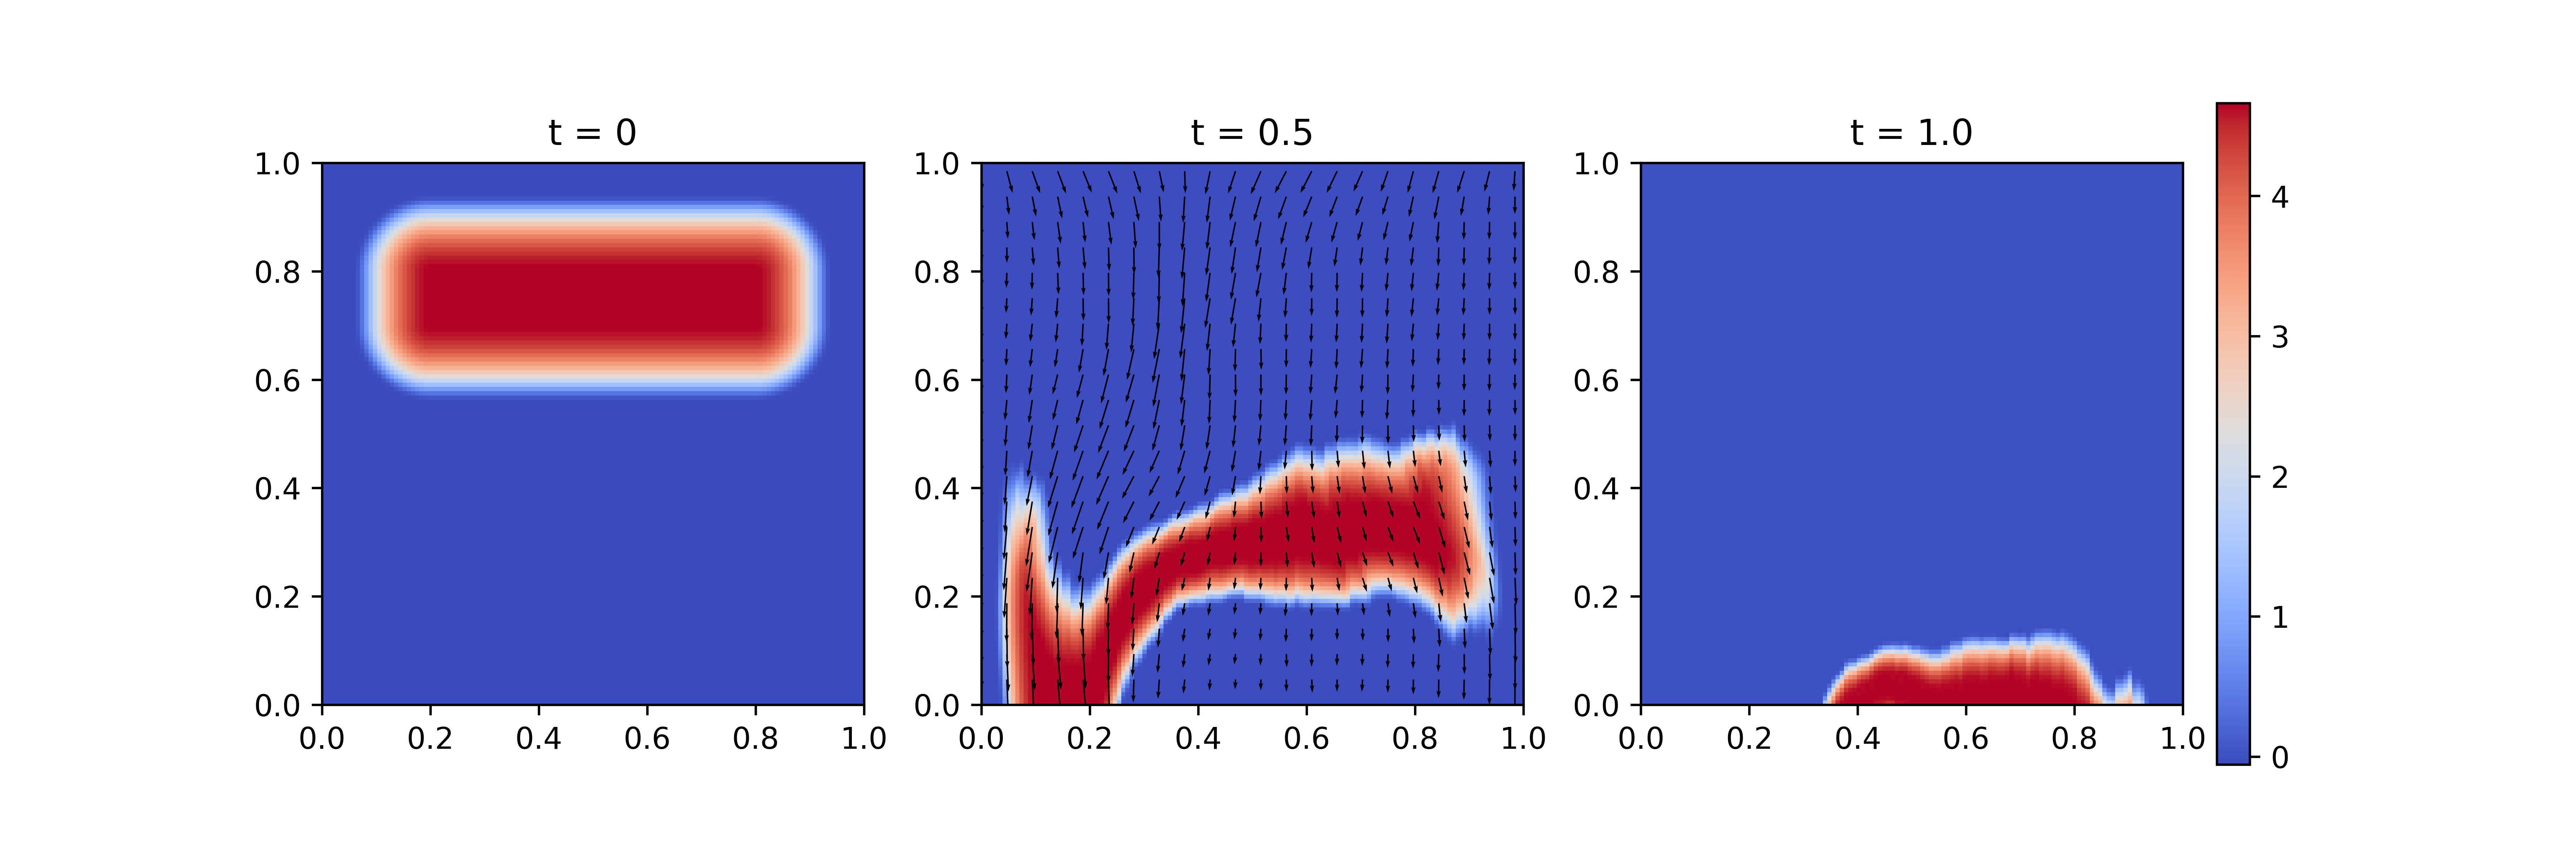
\includegraphics[width=\textwidth]{plots/solution3.png} 
\end{figure}
Die Abbildung links zeigt die Anfangsbedingung zum Zeitpunkt $ t=0 $, in der Mitte ist ein Zwischenschritt der Lösung (zum Zeitpunkt $ t=0.5 $ zu sehen) sowie das zum Sample zugehörige Flussvektorfeld zu sehen. Wir wollen an dieser Stelle noch einmal darauf hinweisen, dass wir das Flussvektorfeld als Lösung eines statischen Problems erhalten. Insbesondere ist also das Flussvektorfeld nicht zeitabhängig und könnte gleichermaßen auch bei Anfangs- und Endzustand eingezeichnet werden. 
Wir berechnen diesen Erwartungswert nun gemäß Abschnitt 6 mit der Multilevel Monte Carlo Methode für die Startwerte $ l_0 = 4, L_0 = 7, N_0 = \{n_4,\dots,n_7\} = \{16,8,4,2\} $und $ \epsilon \in \{0.01,0.005,0.003,0.001\} $.
\subsubsection{Verarbeiten und Darstellen von Vtk-Dateien}
In M++ werden zur Speicherung von Gitterdaten sogenannte Vtk-Dateien genutzt. Alle obigen sowie noch folgende Schaubilder wurden aus diesen Vtk-Dateien generiert. Dafür wurden im Rahmen der Thesis einzelne Module in Python implementiert, welche den Umgang mit diesen Vtk-Dateien erleichtern. 
\begin{figure}[H]
	\centering
	\captionabove{Überblick über implementierte Module}
	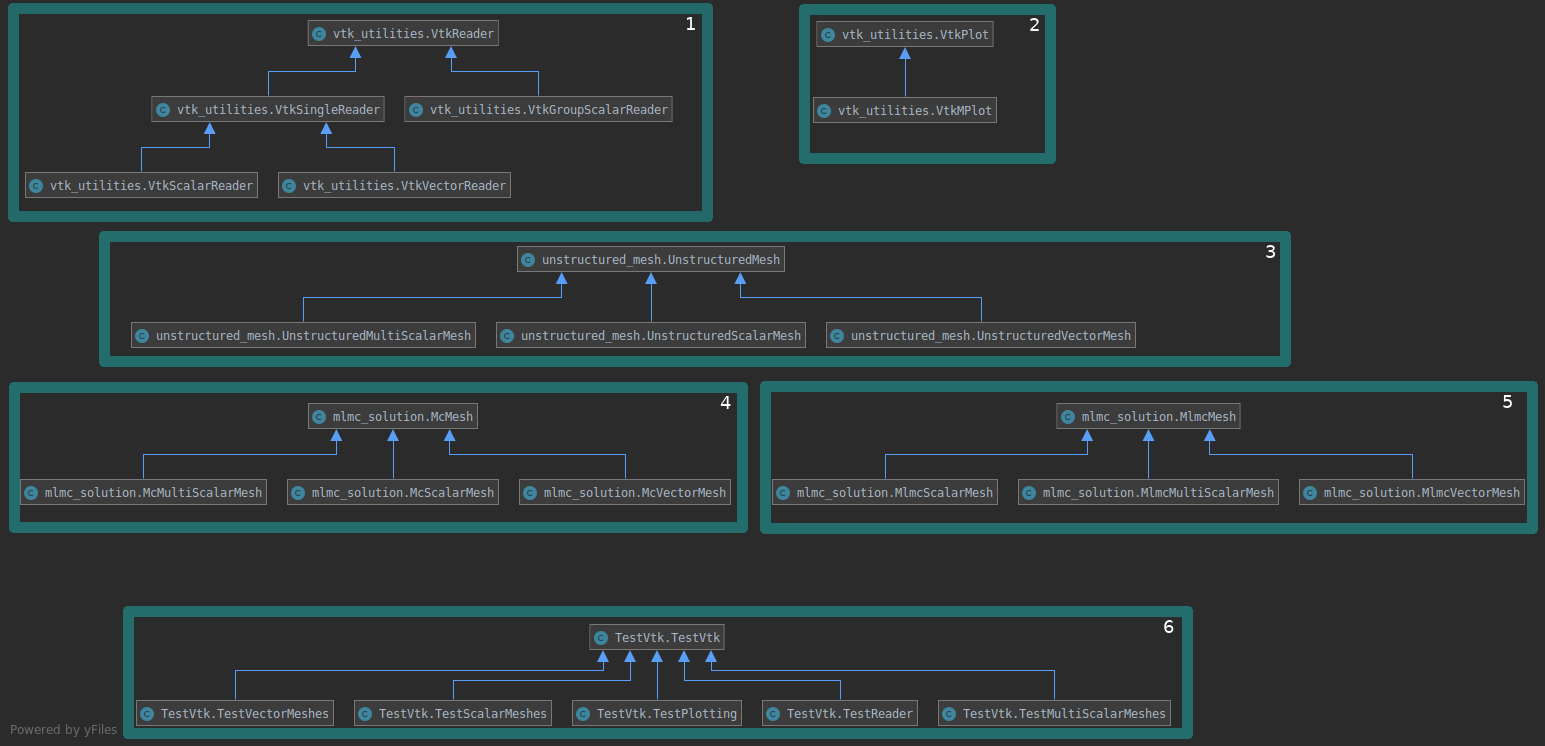
\includegraphics[width=\textwidth]{plots/klassenuml2.png} 
\end{figure}
Wie oben anhand der Klassenstrukturen dargestellt, können die Module in 6 Gruppen unterteilt werden. Gruppe 1 ermöglicht auf Grundlage des externen Moduls 'vtk' \cite{sitevtk} das Lesen von Vtk Dateien. Insbesondere ist es Möglich die Gitterdaten in sogenannten 'numpy-Arrays' zu exportieren. 
Gruppe 2 implementiert ein Interface zum Erstellen verschiedener Schaubilder aus den eingelesen Vtk Dateien. Im später beigefügten Notebook und den entsprechenden Skripten im Hintergrund sind einige exemplarische Beispiele vorhanden. Außerdem wurde alle Schaubilder dieser Thesis über dieses Interface erstellt.
In Gruppe 3 werden die eingelesenen Arrays wieder als 'UnstructuredMesh' aufgefasst. Die Lösungen des Transportproblems selbst besteht aufgrund der Zeitabhängigkeit aus mehreren Gittern. Deshalb fassen wir diese als 'UnstructuredMultiScalarMesh' auf. Das Flussvektorfeld hingegen trägt als Daten Vektoren in jeder Zelle und wird deshalb als 'UnstructuredVectorMesh' betrachtet. Diese objektorientierte Unterteilung zieht sich bis auf Gruppe 2 durch alle Gruppen und ermöglicht den Umgang mit einzelnen Gittern und Skalaren, beispielsweise die Permeabilität des Bodens, mit einzelnen Gittern und Vektordaten, wie etwa das Flussvektorfeld, oder aber einer ganzen Gruppe von Gittern mit Skalaren, womit sich die zeitabhängige Lösung darstellen lässt. Wir können so die Lösungen der Samples als Gitterdaten auffassen und bearbeiten. Insbesondere wurden beispielsweise die Addition und Subtraktion von Gitterdaten implementiert, welche für Generierung von weiteren Gittern nach Vorbild der im Experiment durchgeführten Monte Carlo und Multilevel Monte Carlo Methoden unabdingbar sind. Unter anderem wurde dafür auch eine 'Upscale'-Methode entworfen, welche es ermöglicht unterschiedlich feine Quadratgitter miteinander zu verrechnen.
Gruppe 4 und 5 kombinieren die von M++ während des Experiments abgespeicherten Vtk Dateien wie oben beschrieben. Im Folgenden nennen wir die so (in Form von Gitterdaten) erzeugte Lösung auch 'Mlmc-Lösung'.
Gruppe 6 dient dem Testen der anderen Gruppen in der Form sogenannter 'UnitTests'.
https://github.com/udicr/VtkTools4UnstructeredMeshes.git

\subsection{Ergebnisse}

\subsubsection{Konvergenztest}
\subsubsection{Einige Beispielsamples}
\begin{figure}[H]
	\centering
	\captionabove{Verlauf der Konzentration eines Samples auf Level $ l_0 = 4 $}
	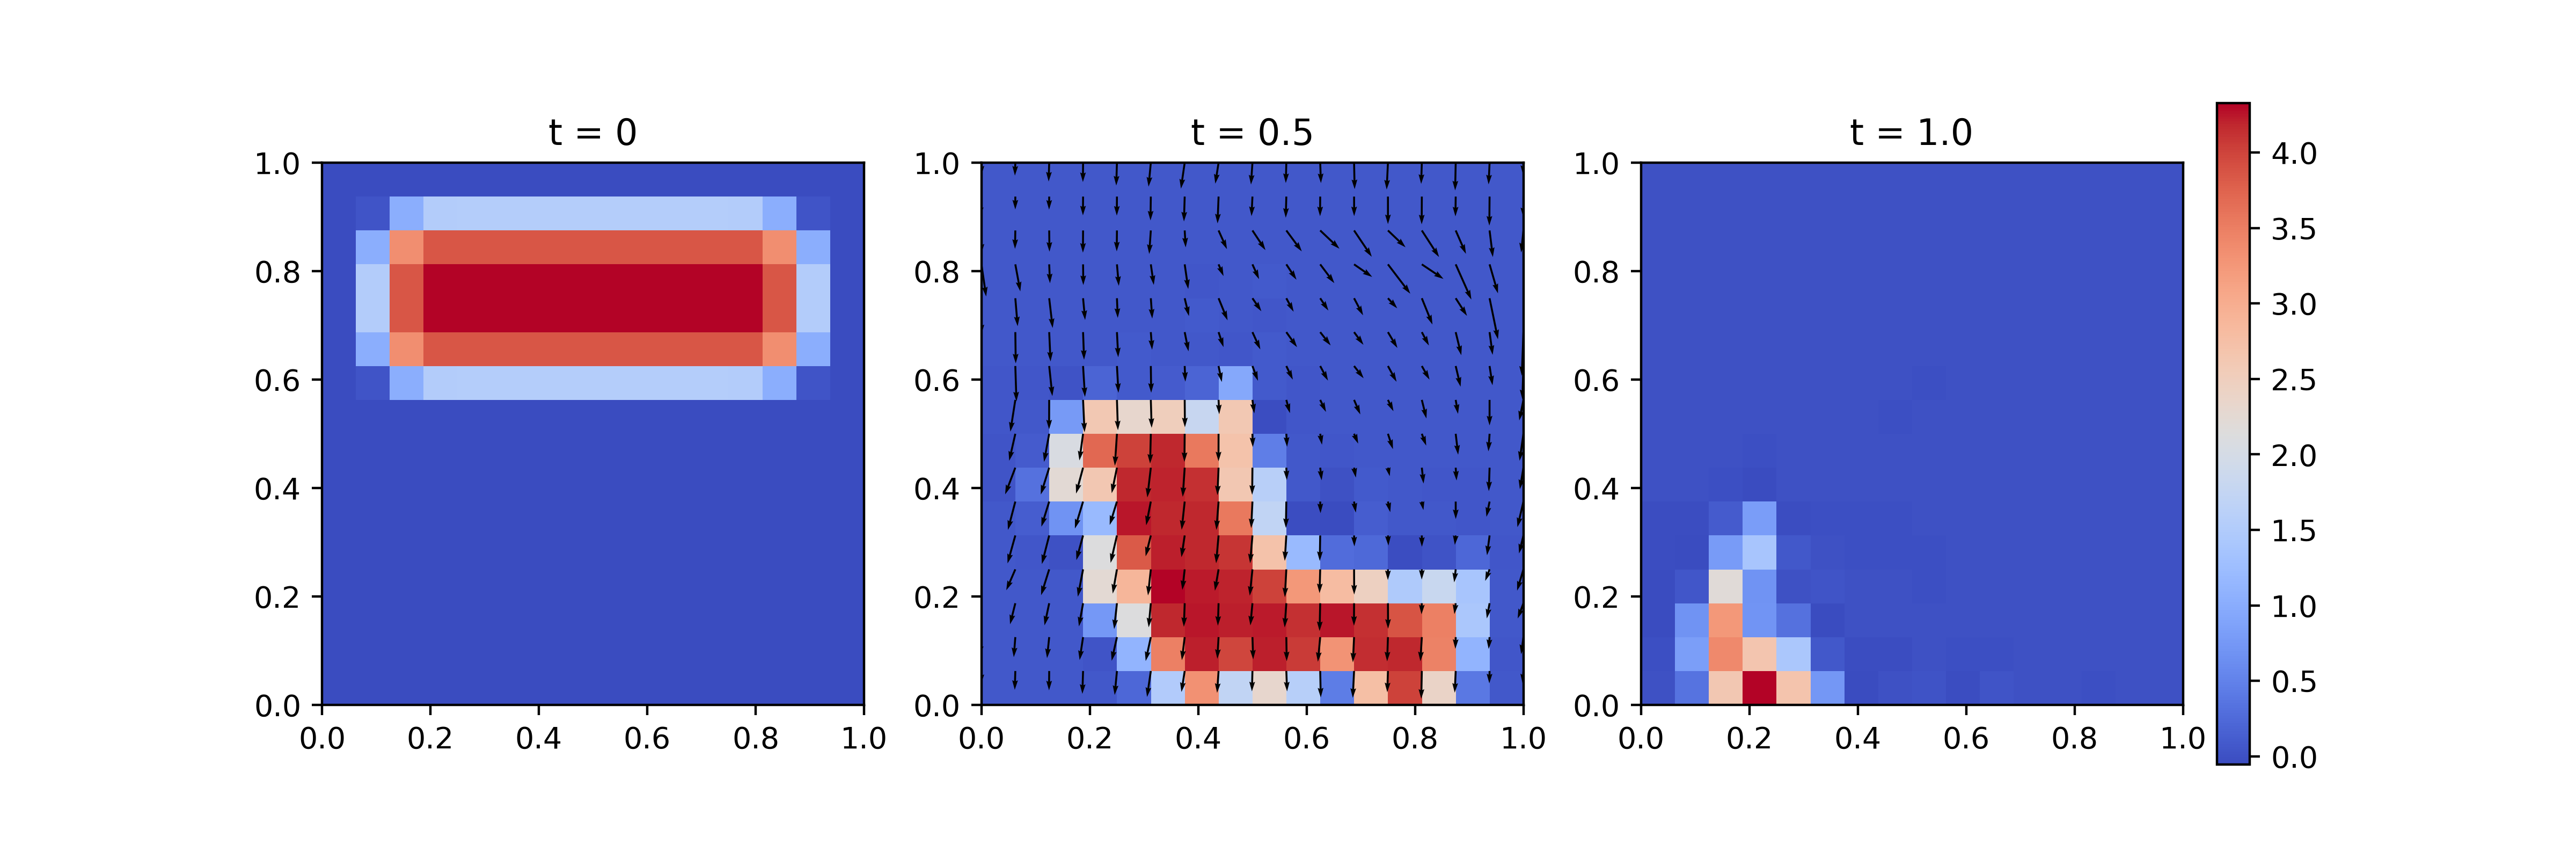
\includegraphics[width=\textwidth]{plots/sample_4_1.png} 
\end{figure}
\begin{figure}[H]
	\centering
	\captionabove{Verlauf der Konzentration eines Samples auf Level $ l_1 = 5 $ und des zugehörigen Vergleichssamples auf Level $ l_0 = 4 $}
	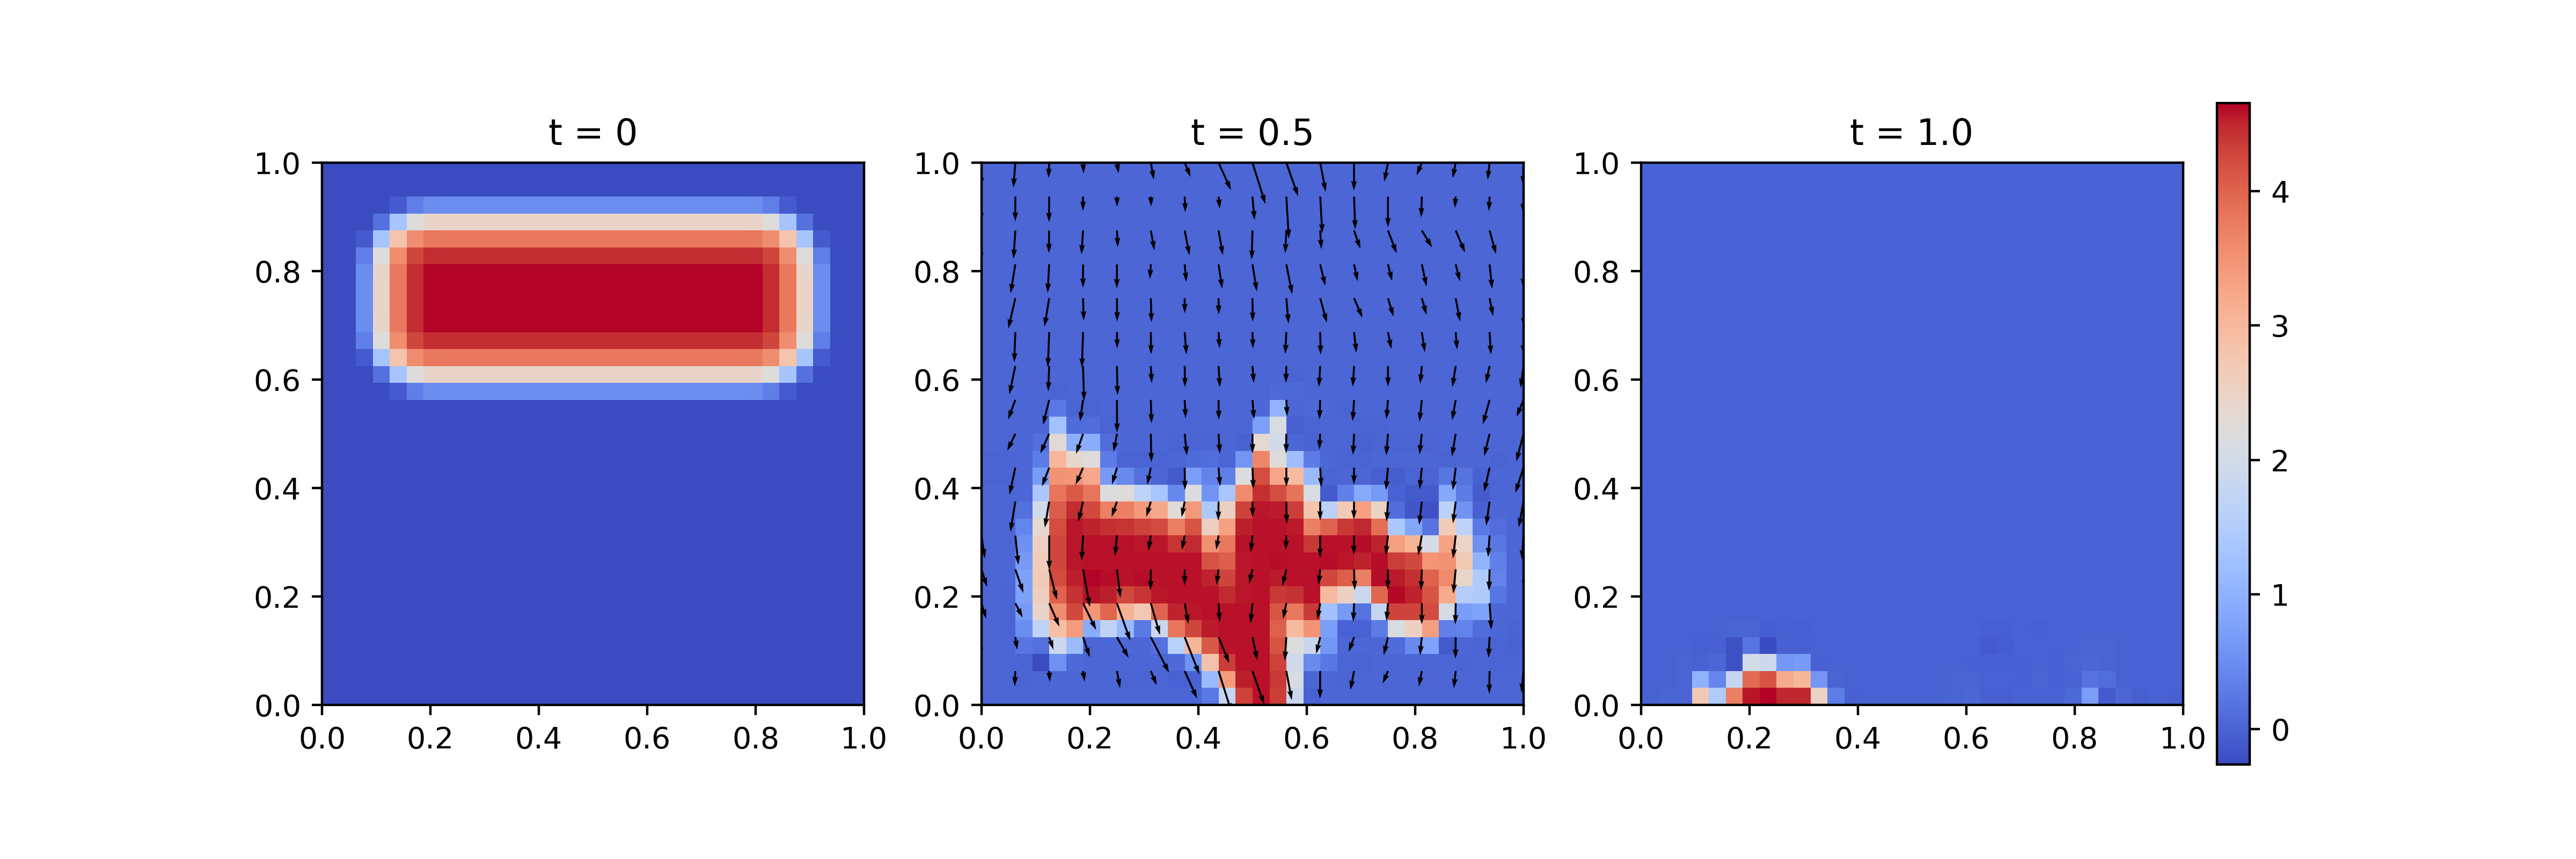
\includegraphics[width=\textwidth]{plots/sample_5_1.png} 
	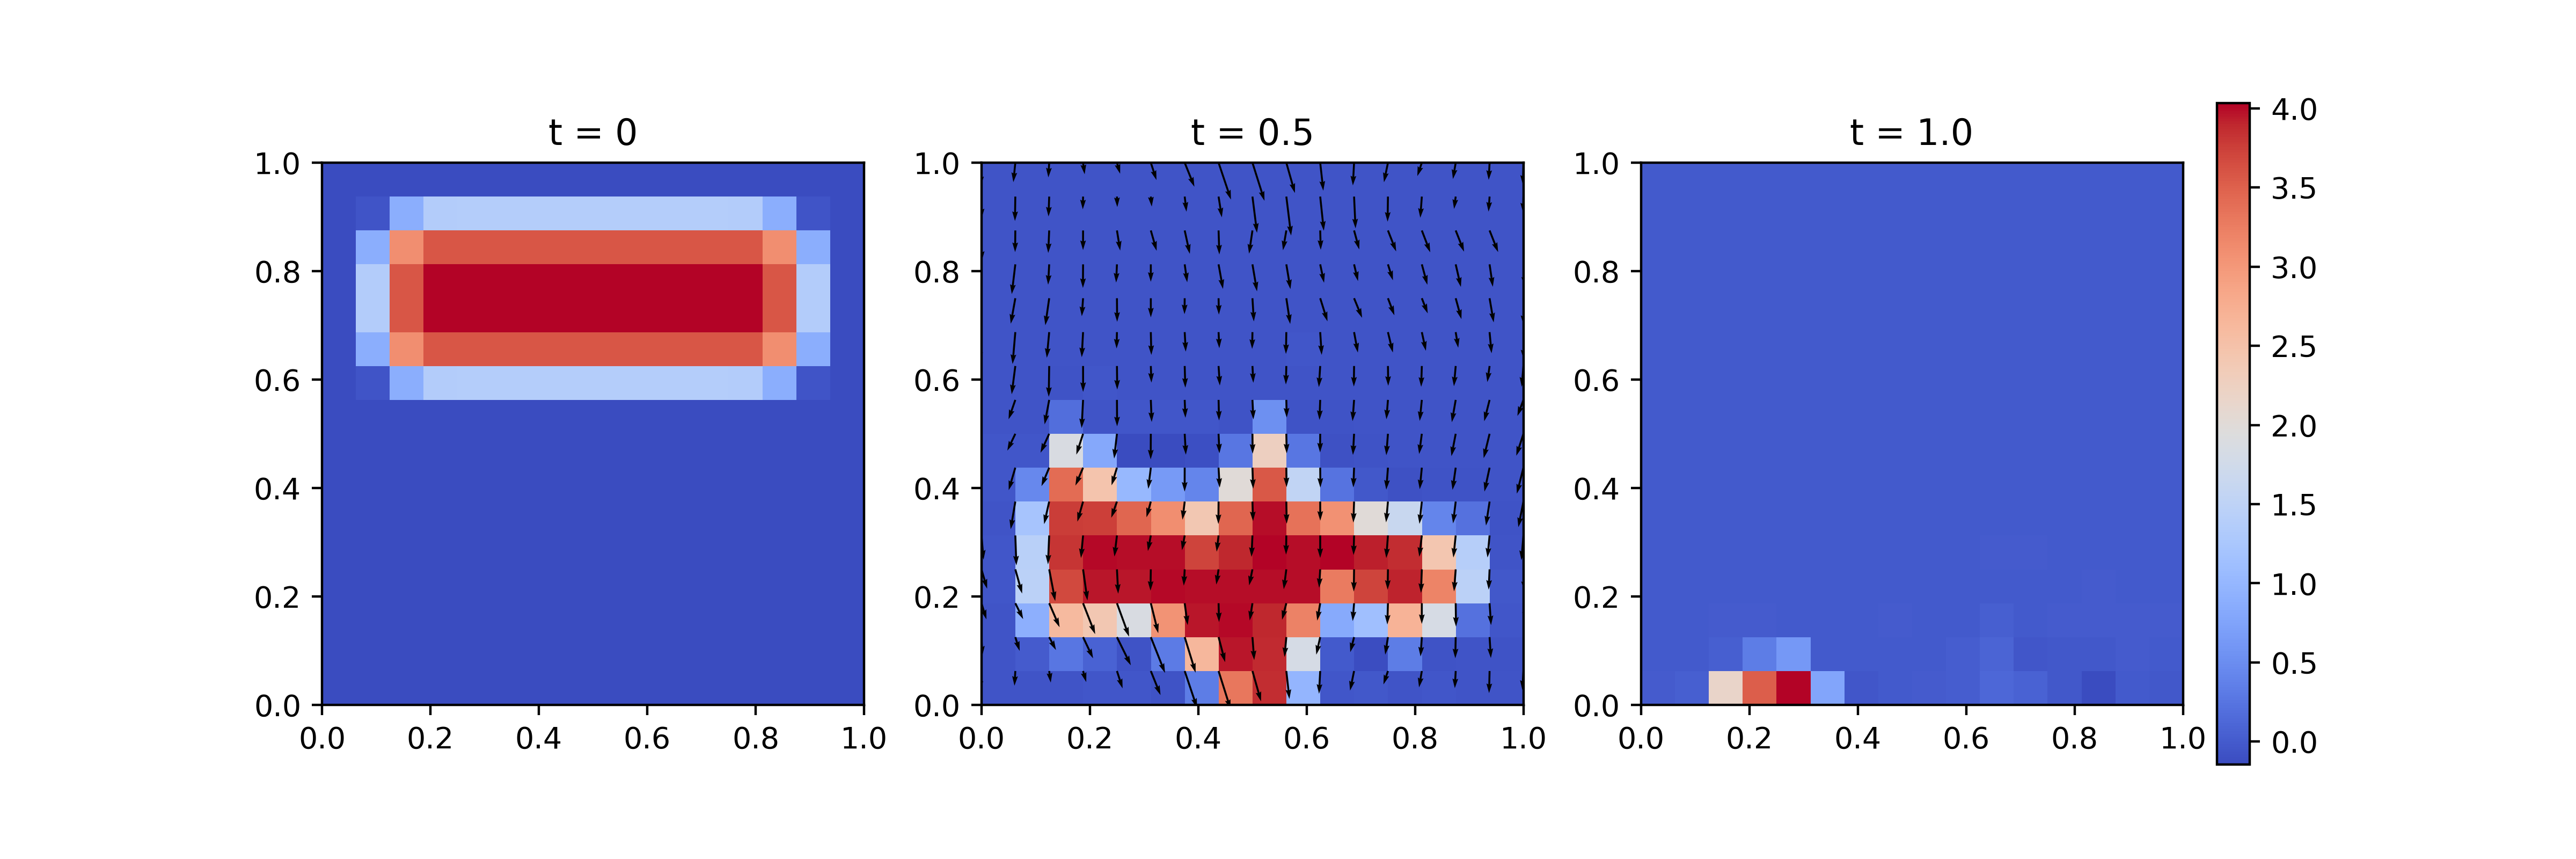
\includegraphics[width=\textwidth]{plots/sample_coarse_5_1.png} 
\end{figure}
An diesem direkten Vergleich sieht man sehr schön, dass sich die beiden Vergleichssamples zwar im Level unterscheiden, aber sich auf dasselbe Zufallsereignis $ \omega_i $ beziehen. Noch offensichtlicher wird das, je höher das aktuell betrachtete Level ist:
\begin{figure}[H]
	\centering
	\captionabove{Verlauf der Konzentration eines Samples auf Level $ l_2 = 6 $ und des zugehörigen Vergleichssamples auf Level $ l_1 = 5 $}
	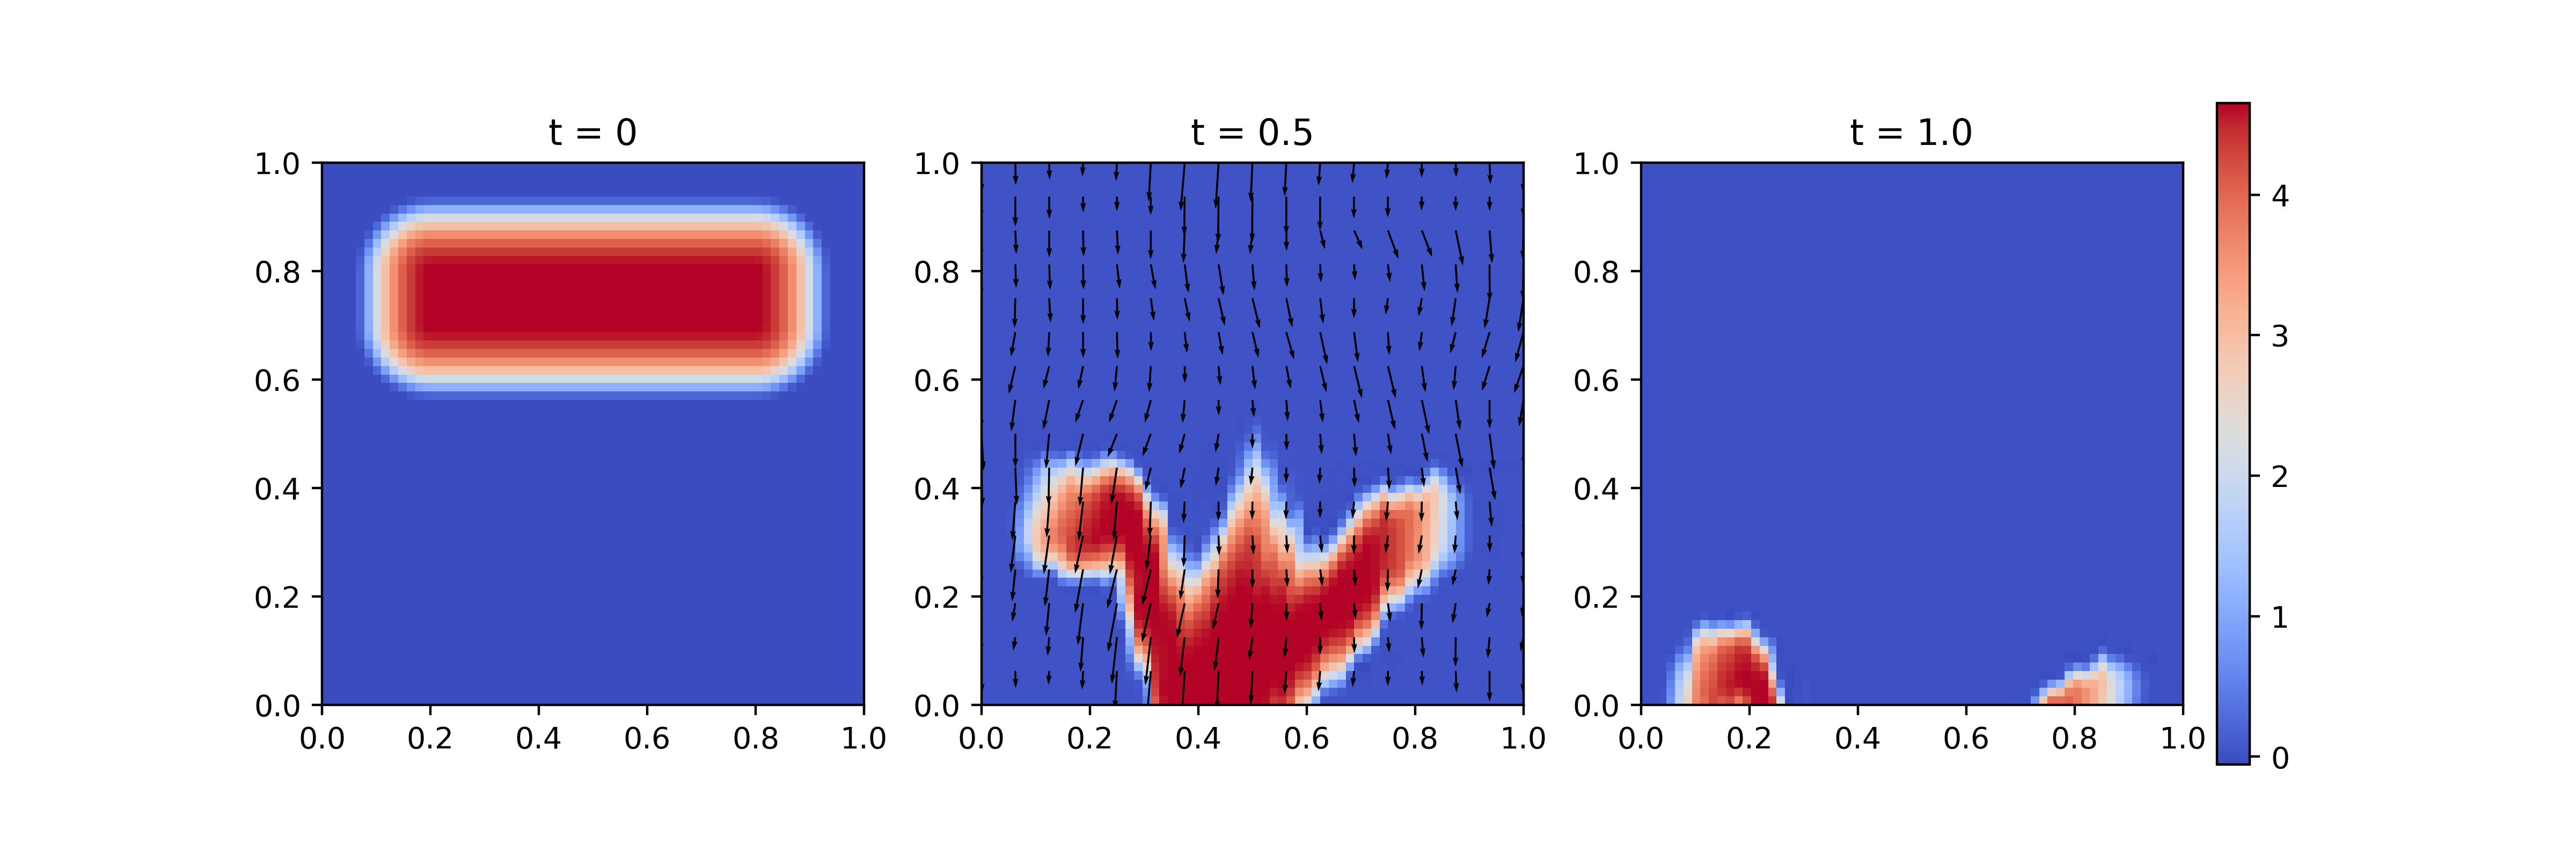
\includegraphics[width=\textwidth]{plots/sample_6_0.png} 
	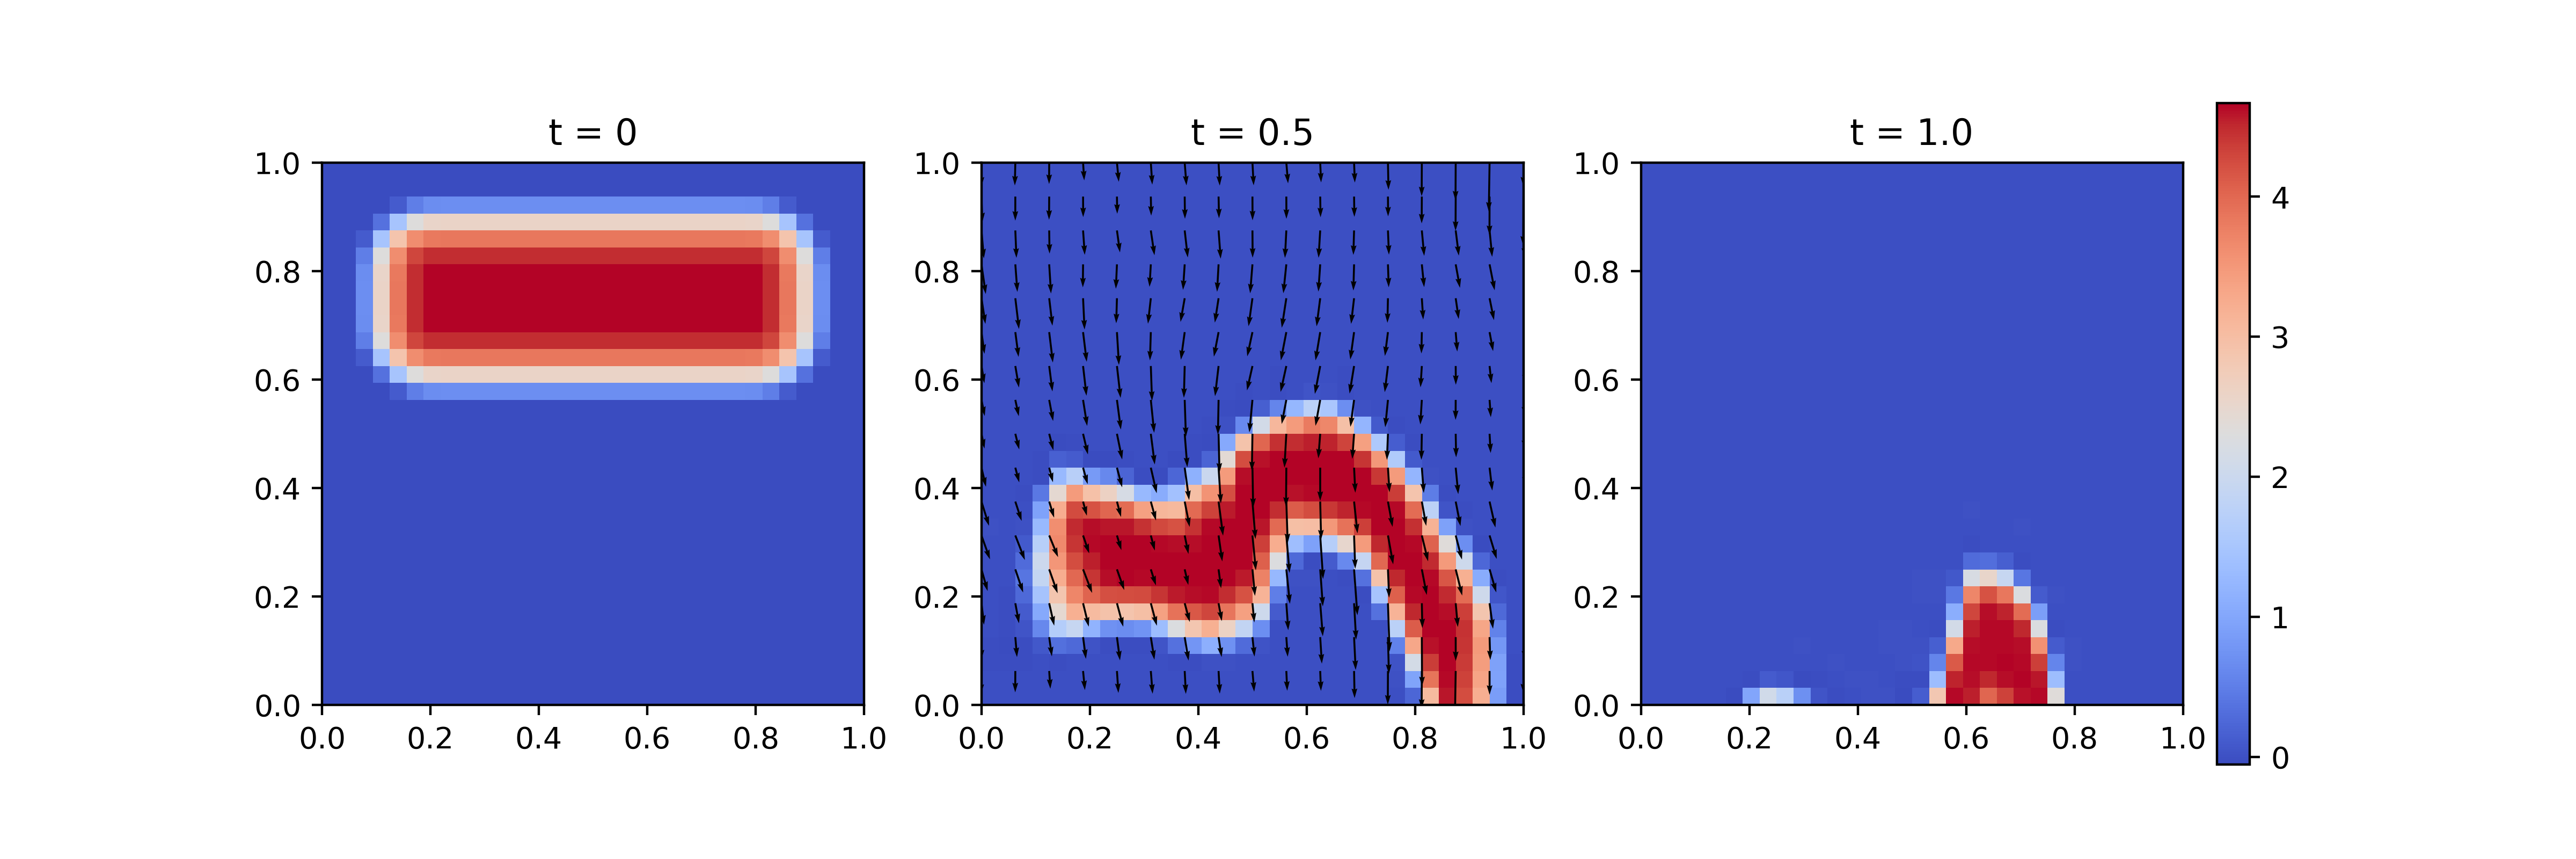
\includegraphics[width=\textwidth]{plots/sample_coarse_6_0.png} 
\end{figure}
\begin{figure}[H]
	\centering
	\captionabove{Verlauf der Konzentration eines Samples auf Level $ l_3 = 7 $ und des zugehörigen Vergleichssamples auf Level $ l_2 = 6 $}
	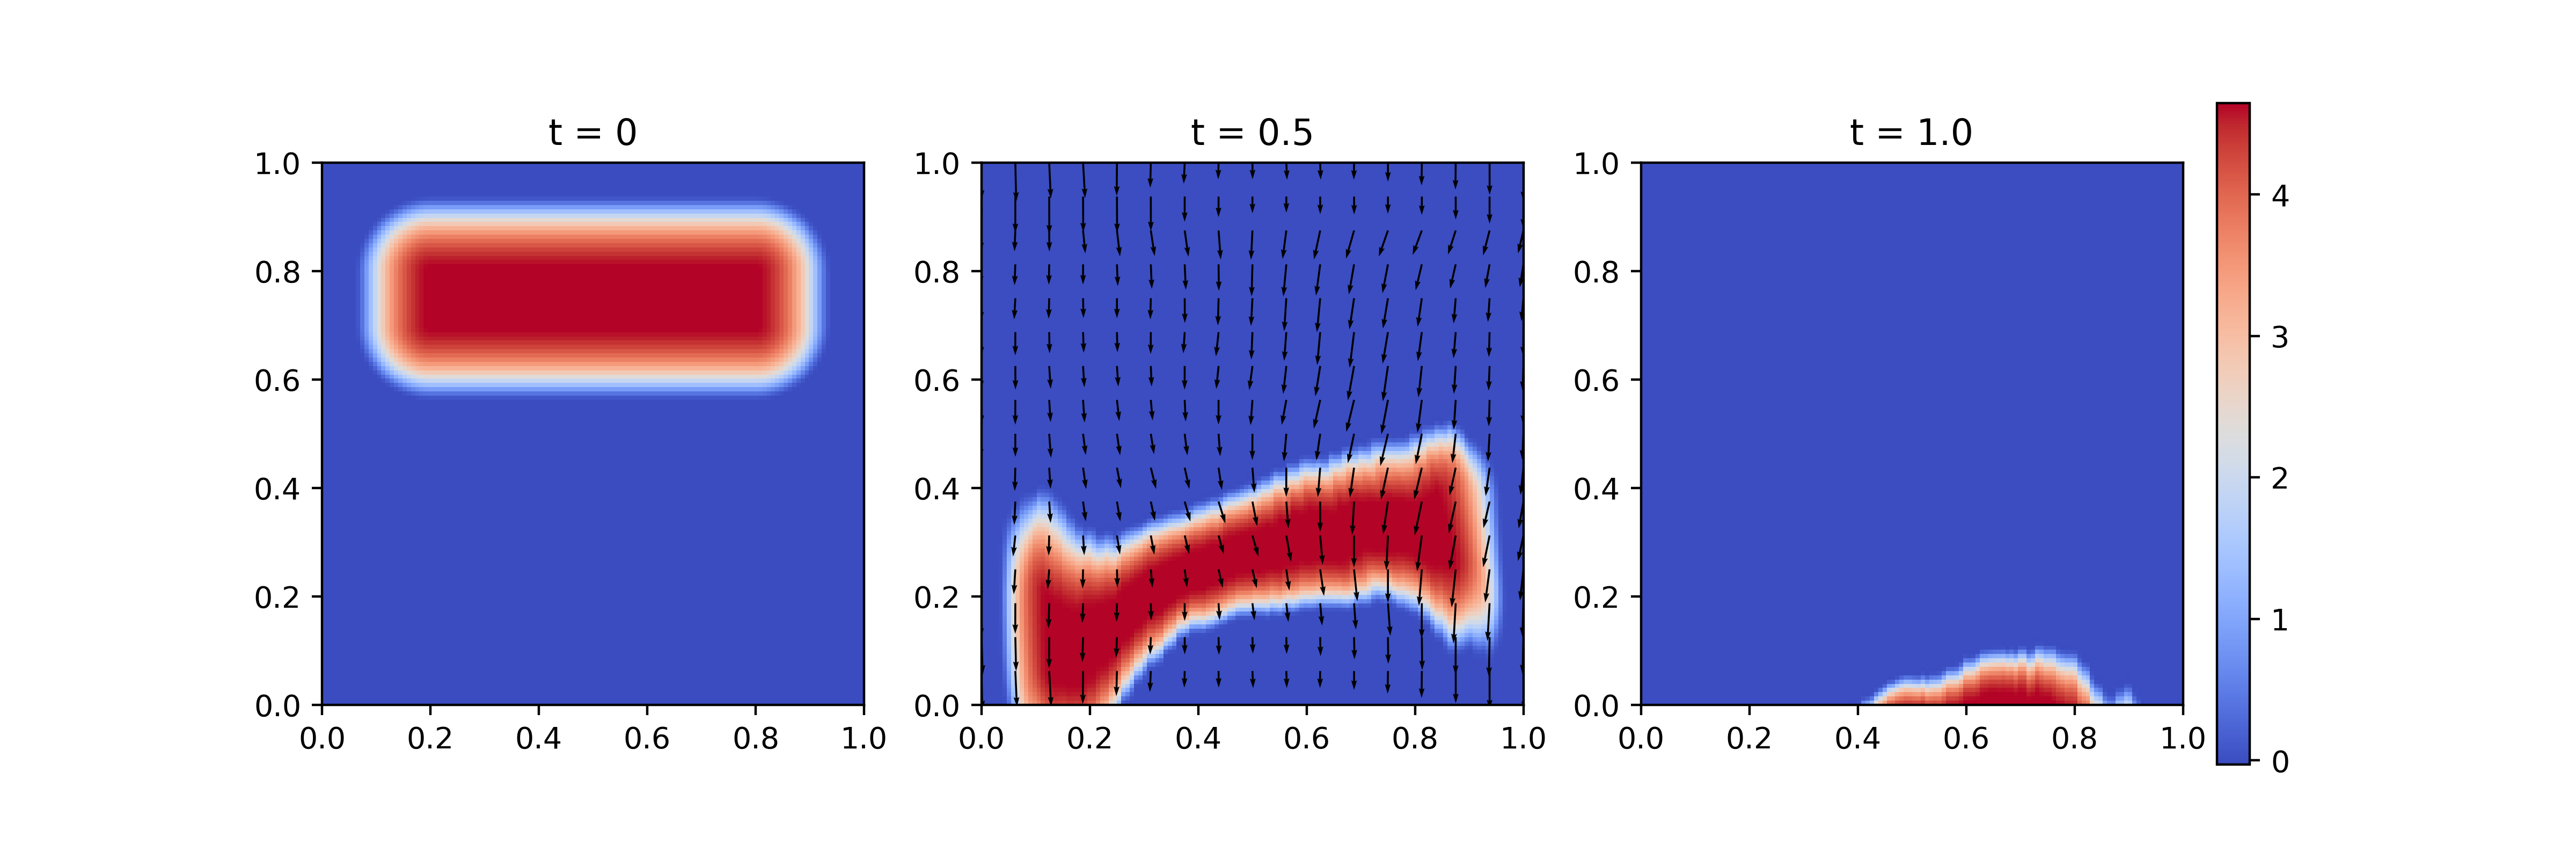
\includegraphics[width=\textwidth]{plots/sample_7_0.png} 
	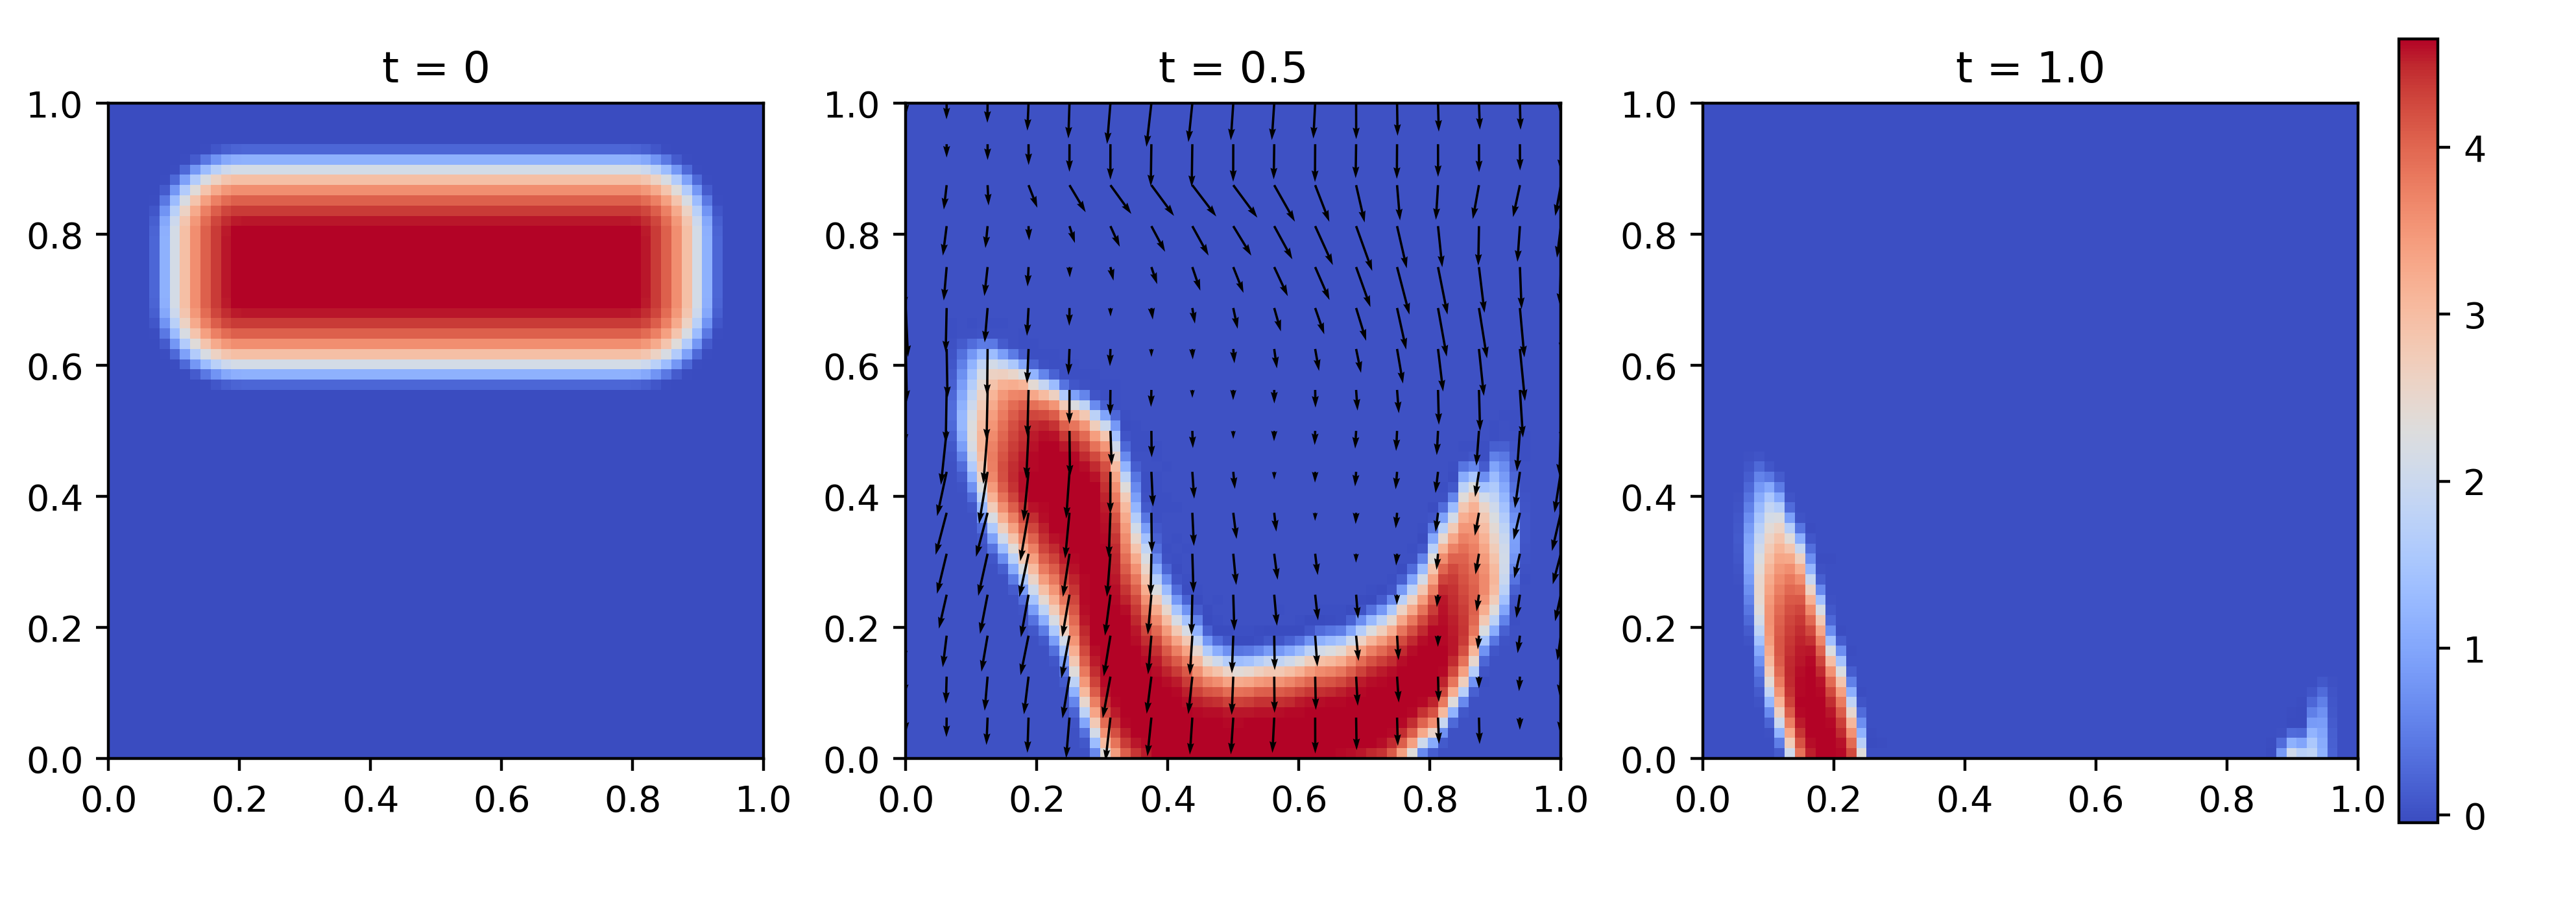
\includegraphics[width=\textwidth]{plots/sample_coarse_7_0.png} 
\end{figure}
\subsubsection{$ \epsilon=0.01 $}
\subsubsection{$ \epsilon=0.005 $}
\subsubsection{$ \epsilon=0.003 $}
\subsubsection{$ \epsilon=0.001 $}
\newlength\q
\setlength\q{\dimexpr .125\textwidth -2.0\tabcolsep}
\noindent\begin{tabular}{|p{0.15\q}|p{0.55\q}|p{1.3\q}|p{1.05\q}|p{1.35\q}|p{1.25\q}|p{\q}|p{1.35\q}|}
\hline
$ l $   &  $ M $  &  $ \mathbb{E}[Q_f-Q_c] $  &   $ \mathbb{E}[Q_f] $ &  $ \mathbb{V}[Q_f-Q_c] $   &   $ \mathbb{V}[Q_f] $ &  kurtosis    &    cost\\
\hline
4 & 60343 &    0.26179  &  0.26179  & 0.0178733   &  0.0178733   &  2.79784 &  294912    \\
5 & 2422  & 0.000190291 &   0.25248 & 0.000231646 &  0.0198675   &  4.85386 & 2.3593e+06 \\
6 & 178   & 0.000974837 & 0.243871  & 9.76543e-06 &  0.0200241   &  3.38187 & 1.88744e+07\\
7 & 12    & 0.000199838 & 0.304479  & 3.18839e-07 &  0.0337465   &   5.9948 & 1.50995e+08\\
8 & 2     & 0.000113336 & 0.0899359 & 1.30611e-08 & 0.00672331   &  32.3407 & 1.20796e+09\\
9 & 2     & 3.5332e-06  & 0.482761  &   1e-10     & 0.000475294  & 0.178766 & 1.07374e+09\\
\hline
\hline
 \multicolumn{2}{|c|}{$ \mathbb{E}[Q] $ }  &  \multicolumn{2}{c|}{MLMC Cost}   & \multicolumn{2}{c|}{$ l $}  &    \multicolumn{2}{c|}{$ M$} \\
\hline
 \multicolumn{2}{|c|}{0.263271} & \multicolumn{2}{c|}{3.32451e+10 } &  \multicolumn{2}{c|}{ 4 5 6 7 8 9  }     & \multicolumn{2}{c|}{60343 2422 178 12 2 2}    \\
\hline 
\hline
\end{tabular}\\
%\begin{tabular}{|c|c|c|c|c|c|c|c|}
%	\hline
%	$ l $   &  $ M $  &  $ \mathbb{E}[Q_f-Q_c] $  &   $ \mathbb{E}[Q_f] $ &  $ \mathbb{V}[Q_f-Q_c] $   &   $ \mathbb{V}[Q_f] $ &  kurtosis    &    cost\\
%	\hline
%	4 & 60343 &    0.26179  &  0.26179  & 0.0178733   &  0.0178733   &  2.79784 &  294912    \\
%	5 & 2422  & 0.000190291 &   0.25248 & 0.000231646 &  0.0198675   &  4.85386 & 2.3593e+06 \\
%	6 & 178   & 0.000974837 & 0.243871  & 9.76543e-06 &  0.0200241   &  3.38187 & 1.88744e+07\\
%	7 & 12    & 0.000199838 & 0.304479  & 3.18839e-07 &  0.0337465   &   5.9948 & 1.50995e+08\\
%	8 & 2     & 0.000113336 & 0.0899359 & 1.30611e-08 & 0.00672331   &  32.3407 & 1.20796e+09\\
%	9 & 2     & 3.5332e-06  & 0.482761  &   1e-10     & 0.000475294  & 0.178766 & 1.07374e+09\\
%	\hline
%	\hline
%	$ \epsilon $  &     $ \mathbb{E}[Q] $  & MLMC cost   & \multicolumn{2}{c|}{$ l $}  &    \multicolumn{3}{c|}{$ M$} \\
%	\hline
%	0.001  &  0.263271 & 3.32451e+10  &  \multicolumn{2}{c|}{ 4 5 6 7 8 9  }     & \multicolumn{3}{c|}{60343 2422 178 12 2 2}    \\
%	\hline 
%	\hline
%\end{tabular} \\
                                                                           \\
Außerdem lassen sich auf Grundlage dieser Daten die Konvergenzparameter und Fehlerkomponenten abschätzen. 
Wir schätzen an dieser Stelle $ \alpha $, also den Exponent der schwachen Konvergenz des Verfahrens, durch lineare Regression der Erwartungswerte $ \mathbb{E}[Q_f - Q_c] $. Anzumerken ist hierbei dass auf dem Basislevel, hier Level 4, keine Differenz in Spalte 3 und 5 angegeben werden kann, da auf dem Basislevel nur einzelne Samples ohne gröberes Vergleichssample betrachtet werden. Stattdessen werden hier in Spalte 3 und 5 ebenfalls wie in Spalte 4 und 6 der einzelne Erwartungswert bzw. die einzelne Varianz angegeben. Bei der Schätzung von $ \alpha $ wird deshalb das Basislevel nicht einbezogen.
Den Exponenten des Rückgangs der Varianz $ \beta $ schätzen wir über den den Rückgang der empirischen Varianzen. Die Kosten in der letzten Spalte selbst werden während des Experiments über die Anzahl der Freiheitsgrade des zugrunde liegenden linearen Gleichungssystems abgeschätzt. 
Auf Grundlage dieser geschätzten Kosten lässt sich auch dann $ \gamma $ bestimmen.
Konkret erhalten wir mit obigen Daten: 
\begin{align*}
	\alpha  &=    1.46067   \\
	\beta   &=    5.18332   \\
	\gamma  &=    2.36601   \\
\end{align*}
Außerdem können wir auch die einzelnen Fehlerkomponenten abschätzen, diese Fehlerschätzung wird auch im Algorithmus selbst vorgenommen. Wir erhalten: 
\begin{align*}
\text{numErr}  &= 6.95372e-05   \quad \text{(geschätzter numerischer Fehler)}\\
\text{statErr} &= 0.000692712  \quad  \text{(geschätzter statistischer Fehler)}\\
\text{error}   &= 0.000762249  \quad  \text{(geschätzter Gesamtfehler)}\\
\end{align*}



\subsection{Notebook}

